%! Author = shenyixiao
%! Date = 13/03/2023
%%%%%%%%%%%%%%%%%%%%%%%%%%%%%%%%%%%%%%%%%%%%%%%%%%%%%%%%%%%%%%%%%%%%%%%%%%%%%%%%%%%%%%%%%%%%%%
%Packages
%%%%%%%%%%%%%%%%%%%%%%%%%%%%%%%%%%%%%%%%%%%%%%%%%%%%%%%%%%%%%%%%%%
\documentclass[12pt, a4paper]{report}
\usepackage{graphicx, listings, framed, mdframed, float}
\usepackage{appendix, pdfpages, setspace, color, hyperref}
\usepackage{tocloft}                    % This squashes the Table of Contents a bit
\hypersetup{colorlinks=true}            % To avoid the borders around hyperlinks
\hypersetup{colorlinks, citecolor=black, filecolor=black, linkcolor=black, urlcolor=black}
\definecolor{MyLightYellow}{cmyk}{0,0.,0.2,0} % Used for program listings
\definecolor{shadecolor}{cmyk}{0,0.2,0,0} % Used for snugshade listings
\usepackage[top=3cm, bottom=3cm]{geometry}
\usepackage{listings}
\usepackage{subcaption}
\usepackage{xcolor}
\usepackage{booktabs}
\usepackage{multirow}
\setlength{\parskip}{10pt}                % sets spacing between paragraphs
\interfootnotelinepenalty=500             % this prevents footnotes breaking across pages
%%%%%%%%%%%%%%%%%%%%%%%%%%%%%%%%%%%%%%%%%%%%%%%%%%%%%%%%%%%%%%%%%%%%%%%%%%%%%%%%%%%%%%%%%%%%%%
%Commands
%%%%%%%%%%%%%%%%%%%%%%%%%%%%%%%%%%%%%%%%%%%%%%%%%%%%%%%%%%%%%%%%%%
\renewcommand\bibname{References}         % to change Bibliography to References
\renewcommand\lstlistlistingname{List of Codes}
\newcommand{\HRule}{\rule{\linewidth}{0.75mm}} % needed on title page


%%%%%%%%%%%%%%%%%%%%%%%%%%%%%%%%%%%%%%%%%%%%%%%%%%%%%%%%%%%%%%%%%%%%%%%%%%%%%%%%%%%%%%%%%%%%%%
%document
%%%%%%%%%%%%%%%%%%%%%%%%%%%%%%%%%%%%%%%%%%%%%%%%%%%%%%%%%%%%%%%%%%
\begin{document}


\begin{center}
	
\includegraphics[width=0.4\textwidth]{fileForWriting/BigCrest}\\ \vspace{15 mm}
	\textsc{\Large Year 2 Project}\\ \vspace{15 mm}
	\doublespace
	\HRule \\ \vspace{8 mm}
	{\huge \bfseries Wearable Sensor}       % <<<< Put your title here
	\\\vspace{4 mm}
	\HRule \\ \vspace{25 mm}

	Name \textsc{Surname1} (ID 2054321)      \\        % <<<< Your names
	Name \textsc{Surname2} (ID 2052234)      \\        % <<<< Your names
	Name \textsc{Surname2} (ID 2052234)      \\        % <<<< Your names
	Name \textsc{Surname2} (ID 2052234)      \\        % <<<< Your names
	Name \textsc{Surname2} (ID 2052234)      \\        % <<<< Your names
	Group 2p23                                 \\        % <<<< Your group number

	\vspace{15mm}
	\emph{Supervised by } Dr Name \textsc{Surname}     % <<<< Your supervisor
	\vfill             % Bottom of the page
	{\large \today}    % today's date
\end{center}

%%%%%%%%%%%%%%%%%%%%%%%%%%%%%%%%%%%%%%%%%%%%%%%%%%%%%%%%%%%%%%%%%%%%%%%%%%%%%%%%%%%%%%%%%%%%%%
%Abstract
%%%%%%%%%%%%%%%%%%%%%%%%%%%%%%%%%%%%%%%%%%%%%%%%%%%%%%%%%%%%%%%%%%
\begin{abstract}
	This document serves as a template to show you how to present and structure your project dissertation. In the interests of uniformity of format, you are asked not to significantly alter the format and layout of this \LaTeX~ document. The chapter names and structure are intended as a guide, and you are welcome to change these as appropriate. While this is not a definitive guide to dissertation writing, it is intended as a guide to assist in documenting and presenting your project work in an academic and professional manner, and reflects the expectations of those in academia and industry who are likely to read your report. Appended to this guide are some real examples of common mistakes that should be avoided.

	Your Abstract is expected to be between 100 and 250 words in length, and should summarise the problem, outline the approach adopted, and summarise the project findings or results. It's the first (and possibly the only) part to be read, and should provide a snapshot of the whole project in 2 or 3 paragraphs.
\end{abstract}



%%%%%%%%%%%%%%%%%%%%%%%%%%%%%%%%%%%%%%%%%%%%%%%%%%%%%%%%%%%%%%%%%%%%%%%%%%%%%%%%%%%%%%%%%%%%%%
%Declaration
%%%%%%%%%%%%%%%%%%%%%%%%%%%%%%%%%%%%%%%%%%%%%%%%%%%%%%%%%%%%%%%%%%
\newpage
\rule{0mm}{30mm}
\centerline{\textbf{Declaration}}

\fbox{\parbox{0.92\textwidth}{I confirm that I have read and understood the University’s definitions of plagiarism and collusion from the Code of Practice on Assessment. I confirm that I have neither committed plagiarism in the completion of this work nor have I colluded with any other party in the preparation and production of this work. The work presented here is my own and in my own words except where I have clearly indicated and acknowledged that I have quoted or used figures from published or unpublished sources (including the web). I understand the consequences of engaging in plagiarism and collusion as described in the Code of Practice on Assessment (Appendix L).}}



%%%%%%%%%%%%%%%%%%%%%%%%%%%%%%%%%%%%%%%%%%%%%%%%%%%%%%%%%%%%%%%%%%%%%%%%%%%%%%%%%%%%%%%%%%%%%%
%Contents
%%%%%%%%%%%%%%%%%%%%%%%%%%%%%%%%%%%%%%%%%%%%%%%%%%%%%%%%%%%%%%%%%%
\newpage \tableofcontents
\newpage \listoffigures
\newpage \listoftables
\newpage \lstlistoflistings        % this is for program listings; if you don't have any, remove this line

\newpage \onehalfspace   %containging titlepage & abstract & declaration & table of contents...
\chapter{Introduction}  %containging backgrounds...


\chapter{Design and Implementation}

\section{Architecture design}

\section{Data transmitting logic}

\section{3D model design} %architecture design
\chapter{Materials and Methods}


\section{Materials}


\subsection{Main component list}
\begin{enumerate}
	\item   Arduino-UNO-Wifi-Rev2: an upgraded version of the standard Arduino Uno board that incorporates several additional features to enhance its functionality.
	In this project, the onboard Wi-Fi module was fully used to provide a wireless communication.
	\item   Grove IMU 9DOF (ICM20600+AK09918): an inertial measurement unit module that integrates three sensors, including an accelerometer, gyroscope, and magnetometer.
	However, this module does not have the function of temperature compensation.
	Additionally, the chip ICM20600 only supports configuring two kinds of IIC addresses.
	Relevant datasheet is shown in Figure~\ref{fig:limited-IIC-address} in Appendix.
	\item   Gravity I2C Multiplexer: a powerful module that allows for the expansion of the I2C bus on Arduino.
	It solves the problem of overlapping IIC address.
	\item   Multi-core screened cable: to ensure the quality of wired communication.
	\item   TP-Link AC1200 Wireless Dual Band Router: to provide a local area network.
	\item   18650 2,600mAh Lithium Rechargeable Batteries: a built-in power source.
	\item   Velcro Brand Adjustable Straps, 25mm x 680mm.
\end{enumerate}


\subsection{Software}
\begin{enumerate}
	\item JetBrains CLion: for socket server programming;
	\item Arduino IDE \& PlatformIO: for Arduino programming;
	\item Autodesk Fusion 360 \& SolidWorks \& SketchUp: for creating 3D models;
	\item Three.js: for front-end programming;
\end{enumerate}


\section{Methods}


\subsection{Arduino: data collection}\label{subsec:data-fetching}
\begin{enumerate}
	\item   Firstly, connect the IIC multiplexer's VCC, GND, SDA, and SCL pins to the respective pins on the Arduino.
	All the cables used were initially of the GROVE type, which was later replaced by screened cables.
	\item   Then, each IMU was connected to one of the I2C multiplexer channels.
	The port setting was saved into the code as portrayed in List~\ref{lst:port-saving}.

	\lstset{language=C++}
	\begin{lstlisting}[caption=Saving the port setting of four IMUs.,    numbers=left,
		firstnumber=22, label={lst:port-saving}]
//port number
enum portConfiguration {
    IMU_LEFT_FEMUR = 2,
    IMU_RIGHT_FEMUR = 6,
    IMU_LEFT_TIBIA = 5,
    IMU_RIGHT_TIBIA = 7
};
	\end{lstlisting}

	\item   After that, install the relevant libraries to drive the hardware components, such as the ``IMU-ICM20600.h'' and ``DFRobot\_I2C\_Multiplexer.h''.
	Due to some reading issues encountered while using the magnetic sensor, the current project only utilized a 6DOF transformation.
	The initialization logic of four IMUs is shown below, where the default data rate for IMU was set to be 100 Hz.

	\lstset{language=C++}
	\begin{lstlisting}[    numbers=left,
		firstnumber=30, caption=Inilizing the multiplexer as well as four IMUs,label={lst:hardware-init}]
I2CMulti.begin();   //init the multiplexer
for (int i = 0; i < 8; i++) {
    if (i == IMU_LEFT_FEMUR
        || i == IMU_RIGHT_FEMUR
        || i == IMU_LEFT_TIBIA
        || i == IMU_RIGHT_TIBIA) {
        I2CMulti.selectPort(i);
        IMU_external.initialize();  //init the IMU
        IMU_external_data[i].filter.begin(100);
        delay(100);
    }
}
	\end{lstlisting}

	\item   After initialization, a calibration process was followed to improve the accuracy and reliability of the IMU's measurements.
	It was achieved by averaging the whole data in the first three freezing seconds.
	Then, future output would be reduced by this average to reduce factors of potential manufacturing variations or sensor drift.
	Relevant code is included in List~\ref{lst:init-arduino} in Appendix.

	\item   To obtain the motion data, the Attitude and Heading Reference System (AHRS) library named Mahony was utilized to generate Euler angles from raw data.
	It is a set of algorithms designed to estimate the attitude and orientation of objects in three-dimensional space using fusion algorithms such as Kalman filter, Madgwick filter, and Mahony filter.
	These tools enable fusing the raw data of IMUs to obtain more accurate, stable, and reliable attitude information.
	The Mahony library, which is a popular sensor fusion algorithm, was selected for the experiment due to its higher computational efficiency.
	Additionally, it contains a 6DOF transformation without using magnetic sensors.

\end{enumerate}


\subsection{Arduino: wireless communication} \label{subsec:5g-network}
\begin{enumerate}
	\item   To enable the built-in Wi-Fi module on Arduino-UNO-Wifi-Rev2, an external library called WiFiNINA was chosen and implemented.
	This library, provided by the official Arduino website, facilitates communication between the microcontroller and the onboard Wi-Fi module through a Serial Peripheral Interface (SPI).
	It also provides some simple examples for studying.
	\item   Initially, the Arduino was connected to a 2.4G network and attempted to establish a connection with a remote server through a handshake process.
	These functions are all included in the library and have been implemented in the kernel.
	\item   Next, a simple const string message was written to one of the Arduino's sockets and sent by the kernel.
	Given that the server was capable of printing any incoming message, the message was finally displayed on the server's console as intended.
	\item   Following this, a stress test was conducted to evaluate the system's capacity to handle a high volume of data.
	This was accomplished by continuously sending an increasing number to the server, which was then printed by the server.
	Meanwhile, the Arduino would also print out the message sent through a serial communication to the computer.
\end{enumerate}


\subsection{Socket server}
\begin{enumerate}
	\item   Based on an example sketch from an online book~\cite{beej-guide}, a simple C\texttt{++} socket server was built to support responding basic HTTP-GET requests.
	\item   Additionally, a multi thread was added to asynchronously save the motion data sent from Arduino.
	\item   To enhance the transmission of motion data to front-end users, a custom JSON encoder was developed to package the raw motion data into a compact and efficient JSON format as List~\ref{lst:json} shows.
	To increase communication rate, the content in such format has been extremely reduced by using abbreviations, where ``L\_F'' represents the motion data of left femur.
	The Euler angles were also abbreviated to ``y'', ``r'', and ``p''.
	Relevant code of the JSON formatter is in List~\ref{lst:json-formatter} in Appendix.
\end{enumerate}

\lstset{
	language=json,
	numbers=left,
	firstnumber=1
}
\begin{lstlisting}[caption={JSON code sent to front-end client.},label={lst:json}]
{
	"L_F": [{
		"y": -0.01,
		"r": 1.82,
		"p": -0.52}],
	"R_F": [{
		...
}
\end{lstlisting}


\subsection{Displaying engine}\label{subsec:engine}

With the tutorial given by official three.js website~\cite{threejs}, a simple static 3D model generator was thus implemented.
However, such basic generator was not flexible enough to rapidly create a specific model, such as humans or birds.
Hence, a function that can generate models according to user customization was developed.
It works like a text operator and user could change his text to modify a corresponding model subsequently.
Relevant results are presented in the next chapter.
In the meantime, the following are the main features of this displaying engine:

%-----------This is a FIGURE-----------------------
\begin{figure}[htbp]
	\centering
	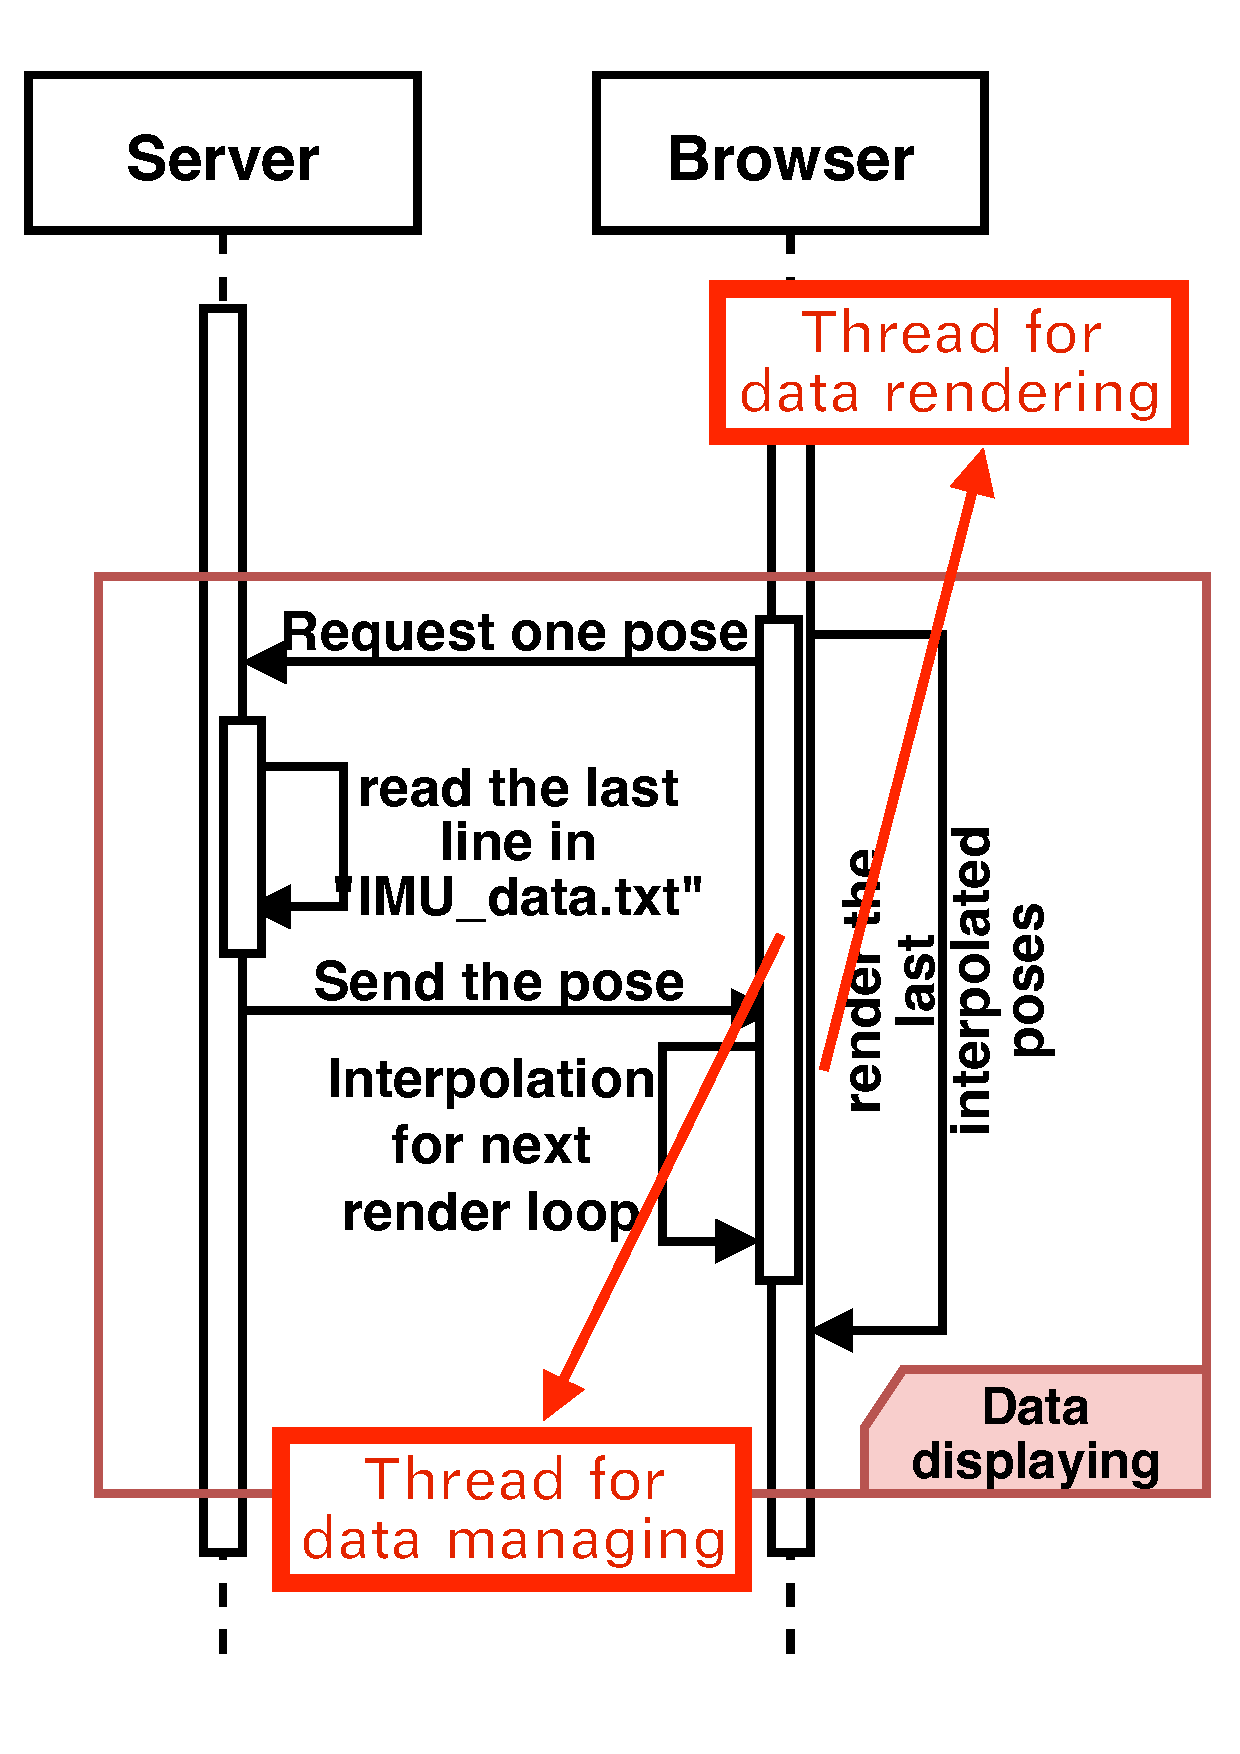
\includegraphics[width=0.5\textwidth]{
		fileForWriting/browser_sequence}
	\caption[Sequence diagram of the displaying engine]{Sequence diagram of the displaying engine.}
	\label{fig:browser_sequence}
\end{figure}
%--------End of this FIGURE -----------


\subsubsection{Reduce latency: multi-thread}
To fully achieve the goal of real time rendering, as depicted by the sequence diagram of Figure~\ref{fig:browser_sequence}, a multi-thread method was also developed.
Particularly, one thread is designed to render the animation, inputting motion data to the model.
Simultaneously, another thread is responsible for managing motion data, requesting them from server and applying interpolation.

By achieving these, the latency raised by data fetching would be reduced to some extent.
Relevant results are shown in the next chapter and core code is shown in
List~\ref{lst:flexible-input} in Appendix.


\subsubsection{Reduce latency: frame interpolation}
To smooth the animation and increase frame rate, a frame interpolation function was also integrated in the thread of data managing.
For example, it would linearly insert five frames into the original single frame.
Relevant core code is shown in List~\ref{lst:intorpolation-with-data-matching} in Appendix.


\subsubsection{Data mapping}
To account for the mismatch between the coordinate system used in the engine and the IMU coordinate system in the real world, a mathematical mapping was also implemented to convert IMU data into angle change values for the animation.

Specifically, for the femur's up and down movements in the engine, the corresponding pitch angle is given by ±(90° + IMU pitch angle), where the positive or negative sign depends on whether the current angle is lifting the leg forward or backward.

During testing, it was observed that the roll output for the femur IMU is usually around 0° when lifting the leg forward, and around 180° when lifting the leg backward.

Given that the yaw data was unstable and useless, the current engine could only achieve the motion follow in vertical plane.
Therefore, a conditional statement using only roll data was added to the program to simply determine whether the leg is being lifted forward or backward.

Relevant core code is shown in List~\ref{lst:intorpolation-with-data-matching} in Appendix, including the data matching for tibia IMU\@.
The logic for tibia IMU is similar but only added its corresponding femur IMU data.
This is because the tibia part in the engine was built from its femur.


\subsubsection{Avoid jittering}
During actual testing, it was found that the model would exhibit some jittering even when the human object was freezing.
Therefore, a threshold limitation feature was added.
Only when the original data's variation exceeds a certain value, the new motion data will be regarded as valid and later input into the model.
Relevant code is shown in List~\ref{lst:intorpolation-with-data-matching} in Appendix.



 %list of all materials, methods?
\chapter{Problem Identification and Resolution}


\section{Issue in network connection}

During the connecting process listed in section~\ref{subsec:5g-network}, it was found that the router had been misconfigured prior to the test.
As a result, the actual LAN was a 5G network, while the built-in Wi-Fi module only supports 2.4G~\cite{arduino_nina_w10_datasheet}.
This was revealed by running an example sketch that scans for all available networks that the Arduino can join.
After that, the unsuccessful LAN was replaced with a cellular network provided by an iPhone, where the Arduino was able to recognize and connect.

%-----------This is a FIGURE-----------------------
\begin{figure}[htbp]
	\centering
	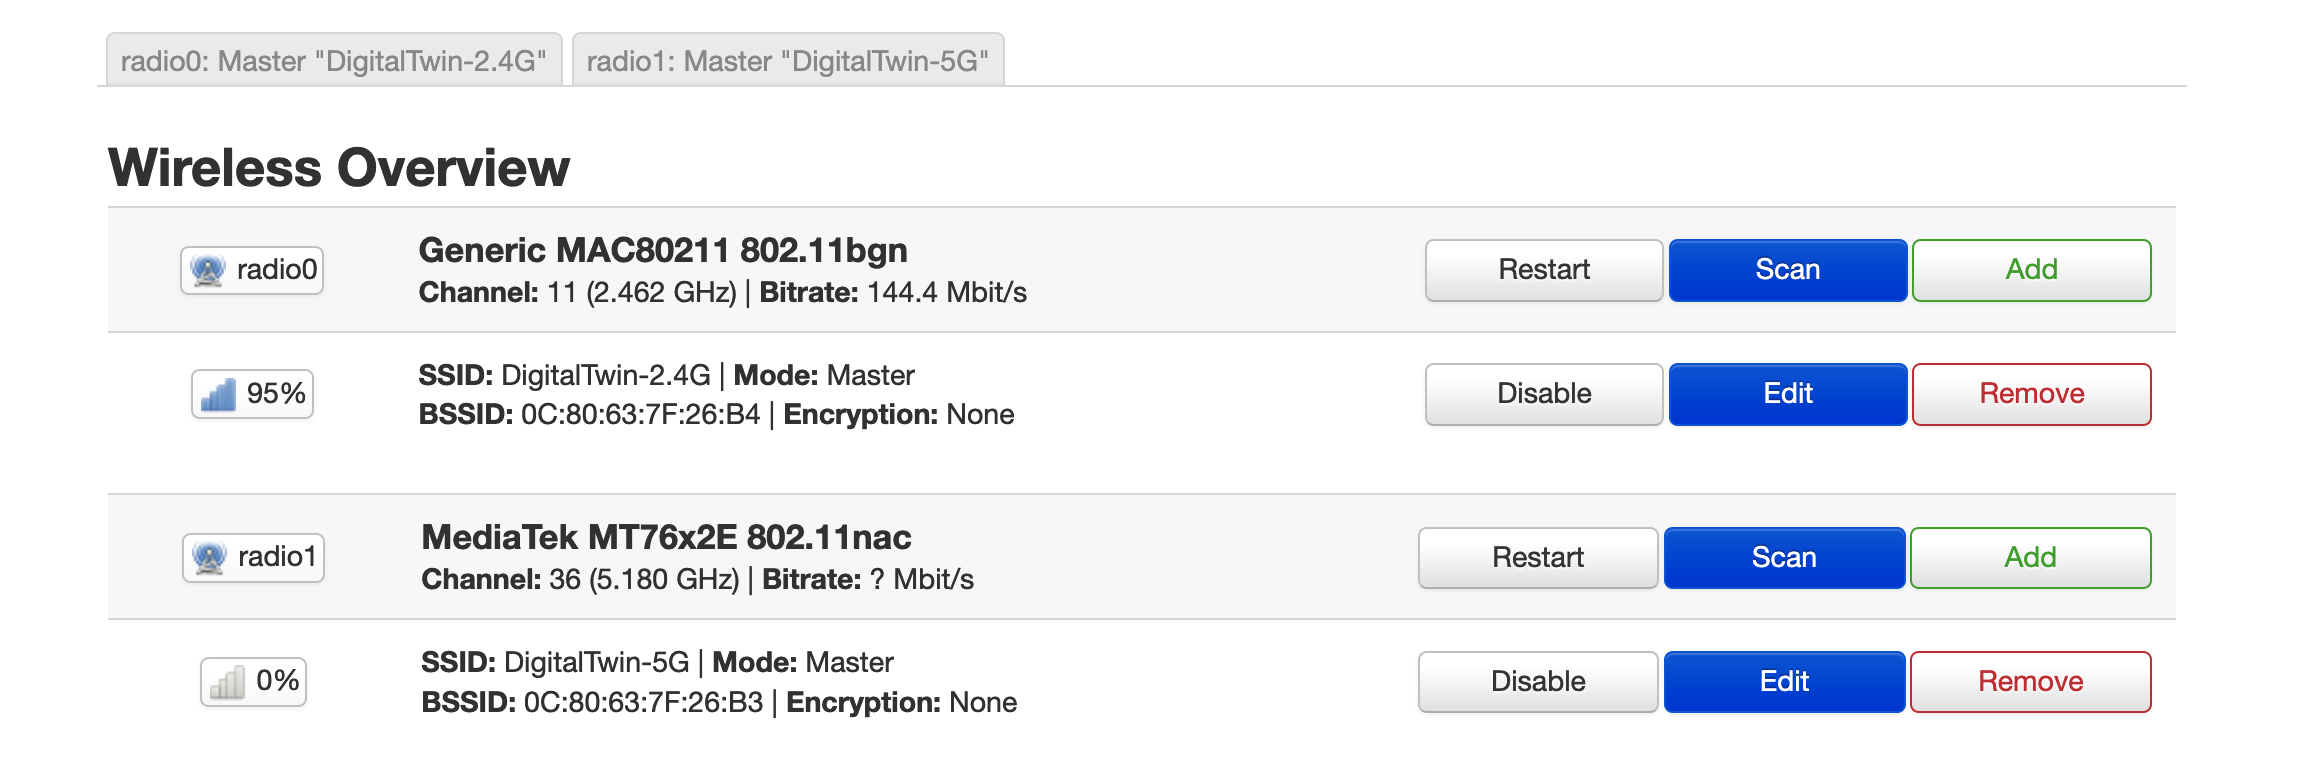
\includegraphics[width=0.8\textwidth]{
		fileForWriting/config}
	\caption[Revised configuration of router]{Revised configuration of router to provide a 2.4G network named ``DigitalTwin-2.4G''.}
	\label{fig:config-5G}
\end{figure}
%--------End of this FIGURE -----------

Such comparison highlighted that the module was working where the router configuration may be improper.
By checking existed configurations and switching the 5G network to 2.4G shown in Figure~\ref{fig:config-5G}, the network provided by the router was eventually recognized and connected by Arduino.

%-----------This is a FIGURE-----------------------
\begin{figure}[htbp]
	\centering
	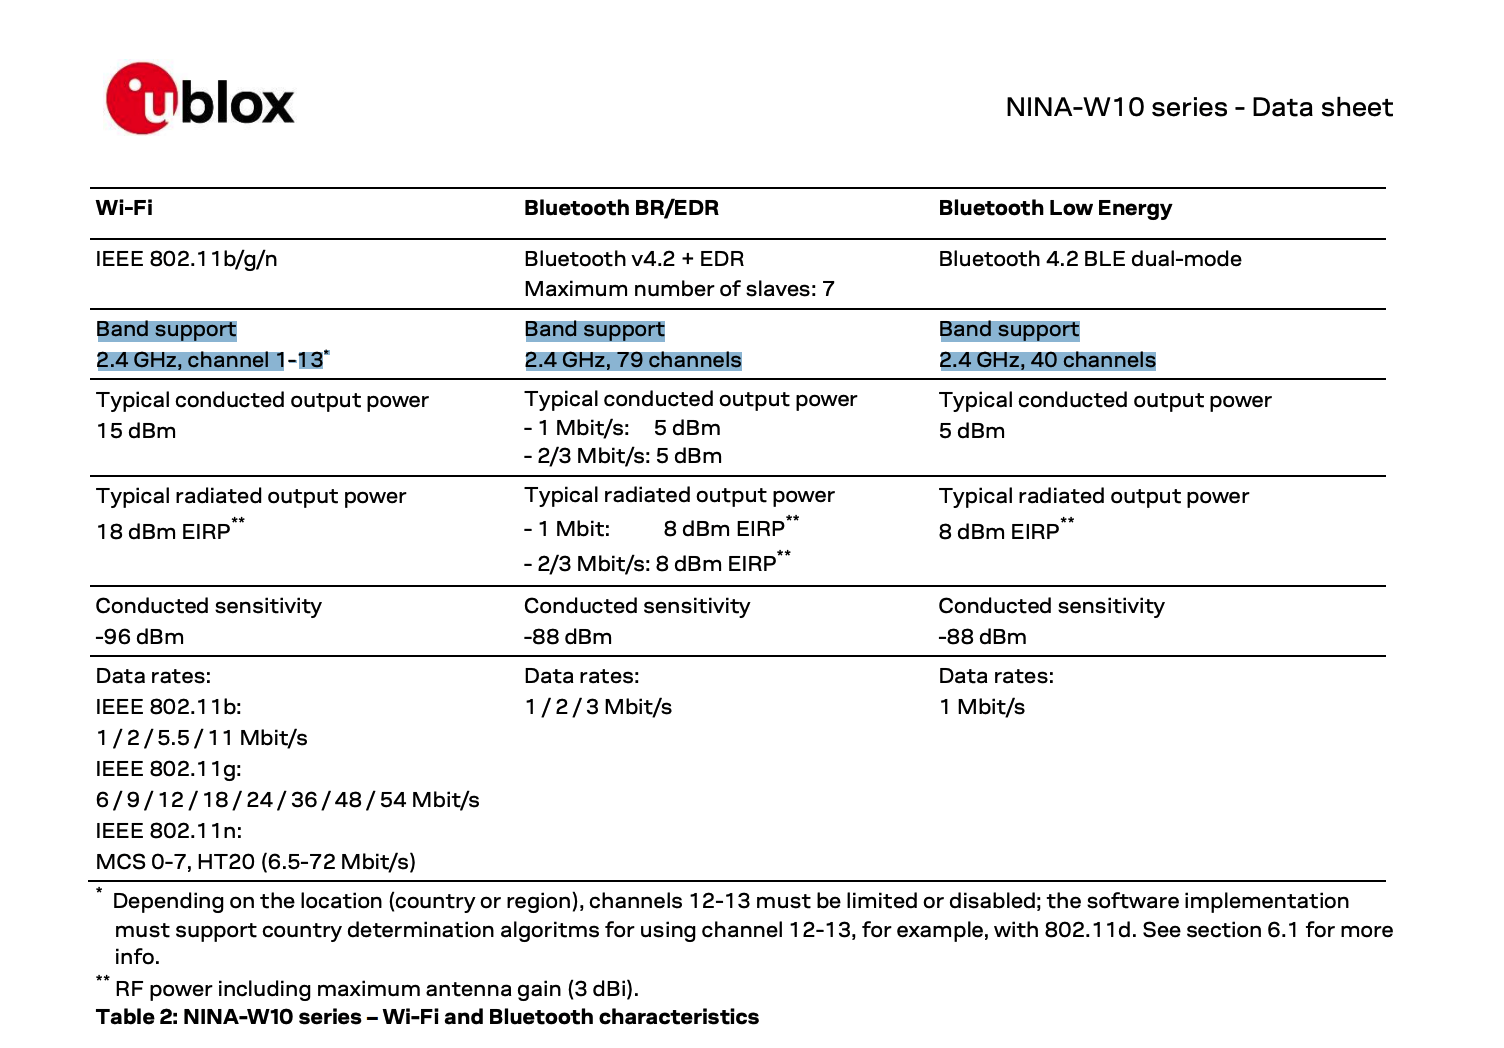
\includegraphics[width=\textwidth]{
		fileForWriting/wifinina}
	\caption[Datasheet of the onboard Wi-Fi module ``NINA-W10'']{Datasheet of the onboard Wi-Fi module ``NINA-W10'', indicating that it only supports the 2.4GHz frequency band.}
	\label{fig:2.4Gonly}
\end{figure}
%--------End of this FIGURE -----------


\section{Issue of ``no socket available''}
\subsection{Problem locating}
During the integration phase, a huge issue was encountered: the Arduino could only send motion data to the server for a very short time (from seconds to at most 3 minutes), where then the built-in Wi-Fi module would throw an error called ``no socket available''.

Although the IMU module and wireless transmission module had passed their own stress tests, an additional stress test for the new framework was subsequently conducted, which involved sending const string messages.
During the test, the Arduino was able to send a const char array continuously without any issues for half hour.
Such stability indicated that the new code framework was not the cause of the problem.

With these three stress tests, this unstable output was eventually identified as ``a function incompatibility between the IMU components and the onboard Wi-Fi component''.


\subsection{Problem analyzing}
Further researching revealed that even though the Wi-Fi module communicates with MCU using SPI protocol, it also has another channel for IIC communication as Figure~\ref{fig:IIC-conflict} has shown.
Such ``additional'' IIC channel is then connected to external IIC channel between the IMU components and MCU\@.
This may have implications for the result of ``no socket available''.

%-----------This is a FIGURE-----------------------
\begin{figure}[htbp]
	\centering
	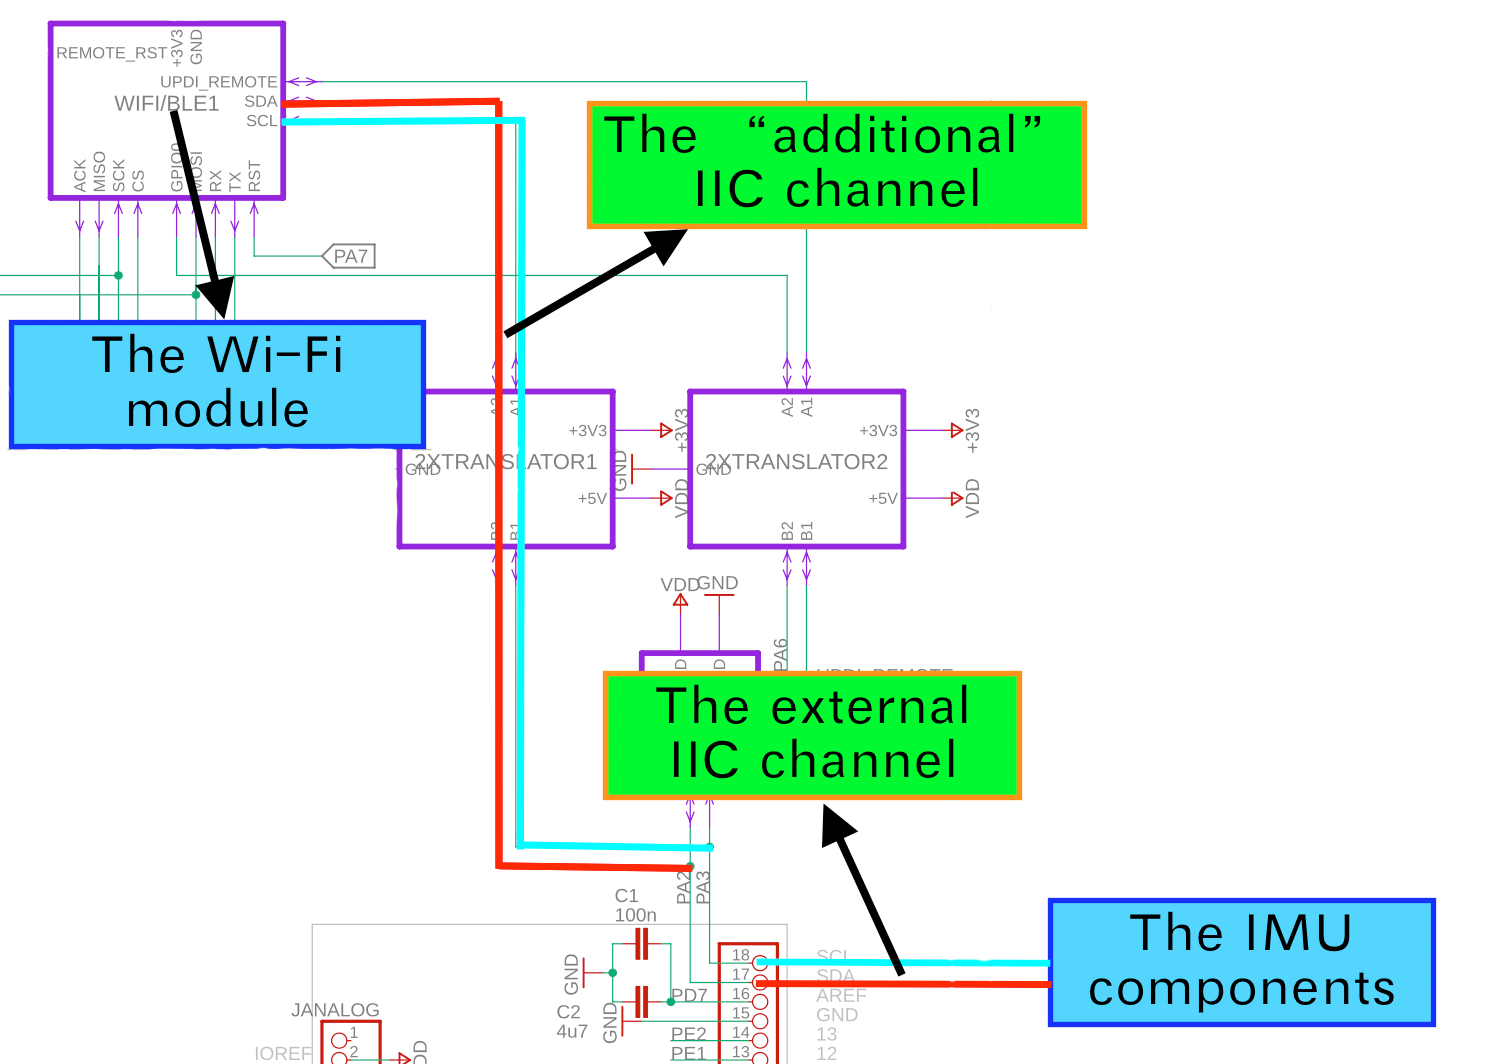
\includegraphics[width=0.8\textwidth]{
		fileForWriting/IIC-conflict}
	\caption[Schematic for the Arduino-UNO-Wifi-Rev2]{Partial schematic for the Arduino-UNO-Wifi-Rev2, where the MCU, Wi-Fi module, and IMUs are sharing a same I2C communication channel.
	}
	\label{fig:IIC-conflict}
\end{figure}
%--------End of this FIGURE -----------



Based on such troubleshooting, a hypothesis was formed that the external I2C might have an impact on the internal I2C, which could then result in a ``no socket available'' error in the Wi-Fi module.
Additionally, during testing, it was noticed that shaking the IMU could subsequently trigger the error.
It was speculated that the internal I2C requires a high level of communication quality.
Hence, one possible solution is improving the poor cables shown in the Figure~\ref{fig:IIC-connections} (a).


\subsection{Problem solving}
\subsubsection{Improve IIC communication quality}

To prevent potential problems raised by poor IIC communication quality, a multicore screened cable was therefore applied, as Figure~\ref{fig:IIC-connections} (b) may show.
Successfully, the Arduino could now continuously send motion data to remote server.


\begin{figure}[htbp]
	\centering
	\begin{subfigure}[b]{0.45\textwidth}
		\centering
		\includegraphics[width=\textwidth]{fileForWriting/original-connection}
		\caption{Original connection using dupont line.}
	\end{subfigure}
	\hfill
	\begin{subfigure}[b]{0.45\textwidth}
		\centering
		\includegraphics[width=\textwidth]{fileForWriting/improved-connection}
		\caption{Improved connection using screened cable.}
	\end{subfigure}
	\caption[]{Two connections of external IIC channel.}
	\label{fig:IIC-connections}
\end{figure}

\subsubsection{Remove the ``additional'' IIC channel}
During the following week of testing, the issue did not reoccur.
However, after several accidental drops of the device, the problem resurfaced and the Arduino could not stably send motion data to server.

To solve the issue from root, the ``additional'' IIC channel was physically removed by desoldering two resistor on that channel as Figure~\ref{fig:remove-IIC} may show.
As expected, the Wi-Fi module was indeed functioning well without any interference from external IIC channel.
This success also proved the correctness of previous analysis.


In summary, the Wi-Fi module is very vulnerable to any external interference in its IIC channel.
If affected, it may stop working and throw a ``no socket available'' error.
As the MCU and module use another SPI channel to communicate, we decided to physically remove that IIC channel since this project did not require an IIC functionality of that module.
After the removal, the whole system worked perfectly.
The root of such issue may be the design flaw of Arduino-UNO-Wifi-Rev2, where the MCU, Wi-Fi module, and external IIC devices directly share one IIC channel.
Simultaneously, the Wi-Fi module may require a high level of communication quality.


%-----------This is a FIGURE-----------------------
\begin{figure}[htbp]
	\centering
	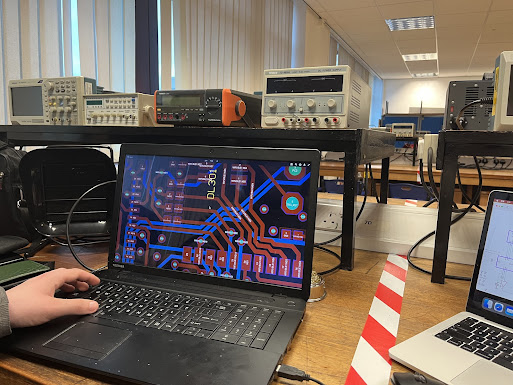
\includegraphics[width=0.7\textwidth]{
		fileForWriting/remove IIC}
	\caption{Desoldering two resistors on the ``additional'' IIC channel to completely solve the ``no socket available'' issue.}
	\label{fig:remove-IIC}
\end{figure}
%--------End of this FIGURE -----------







 %list of all materials, methods?
\chapter{Results}


\section{Arduino: Euler angle output}
Based on the information presented in List~\ref{lst:time-consuming} (see Appendix) in the case of using four IMUs, the data collection interval of each round was about 55ms, nearly 20hz.

Meanwhile, it also turned out that the output of yaw axis data was unstable and inaccurate.
Due to the time limitation, such data was discarded, leading to a loss of some functions for this project.
As a replacement, the roll axis data was used to identify the pitch angle, which has been illustrated in the data mapping part of~\ref{subsec:engine}.

\section{Displaying engine: flexible configuration}\label{sec:flexible}
\begin{figure}[htbp]
	\centering
	\begin{subfigure}[b]{0.45\textwidth}
		\centering
		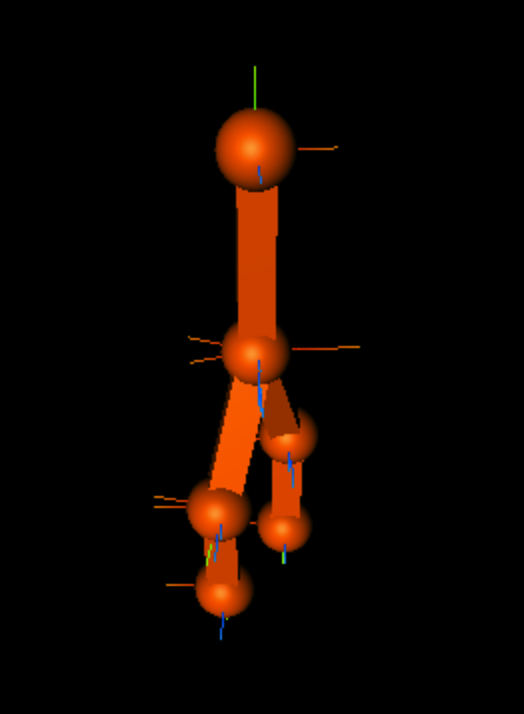
\includegraphics[width=0.8\textwidth]{
			fileForWriting/ouput-model}
		\caption[The model generated by the input text for human lower body]{A human lower body model generated by the input text in List~\ref{lst:lower-body-config}.}
		\label{fig:lower-body-model}
	\end{subfigure}
	\hfill
	\begin{subfigure}[b]{0.45\textwidth}
		\centering
		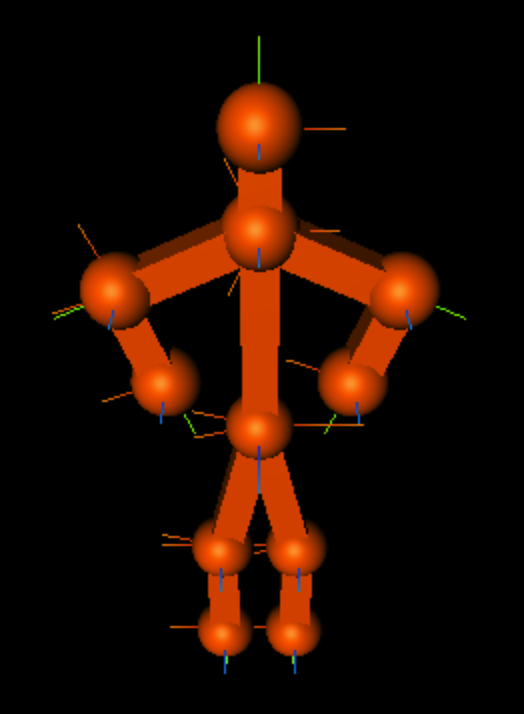
\includegraphics[width=0.8\textwidth]{
			fileForWriting/full-body}
		\caption[The model generated by the input text for a full human body]{A full human body model generated by the input text in List~\ref{lst:full-body-config}.}
		\label{fig:full-body-model}
	\end{subfigure}
	\caption[]{Corresponding models generated by various text inputs in the displaying engine.}
	\label{fig:flexible-input}
\end{figure}

As depicted in Figure~\ref{fig:flexible-input}, with different text inputs, the displaying engine could generate corresponding models.
The Figure (b) is based on the input of Figure (a) but adds other parts such as arms, forearms.
Relevant configs are in List~\ref{lst:lower-body-config} and  List~\ref{lst:full-body-config}.




\section{Displaying engine: asynchronously fetching data}\label{sec:async}
As highlighted by the representation of Figure~\ref{fig:0.73-size}, the thread for data fetching needed about 2 frame intervals to obtain the whole 0.73 MB data from the server.

%-----------This is a FIGURE-----------------------
\begin{figure}[htbp]
	\centering
	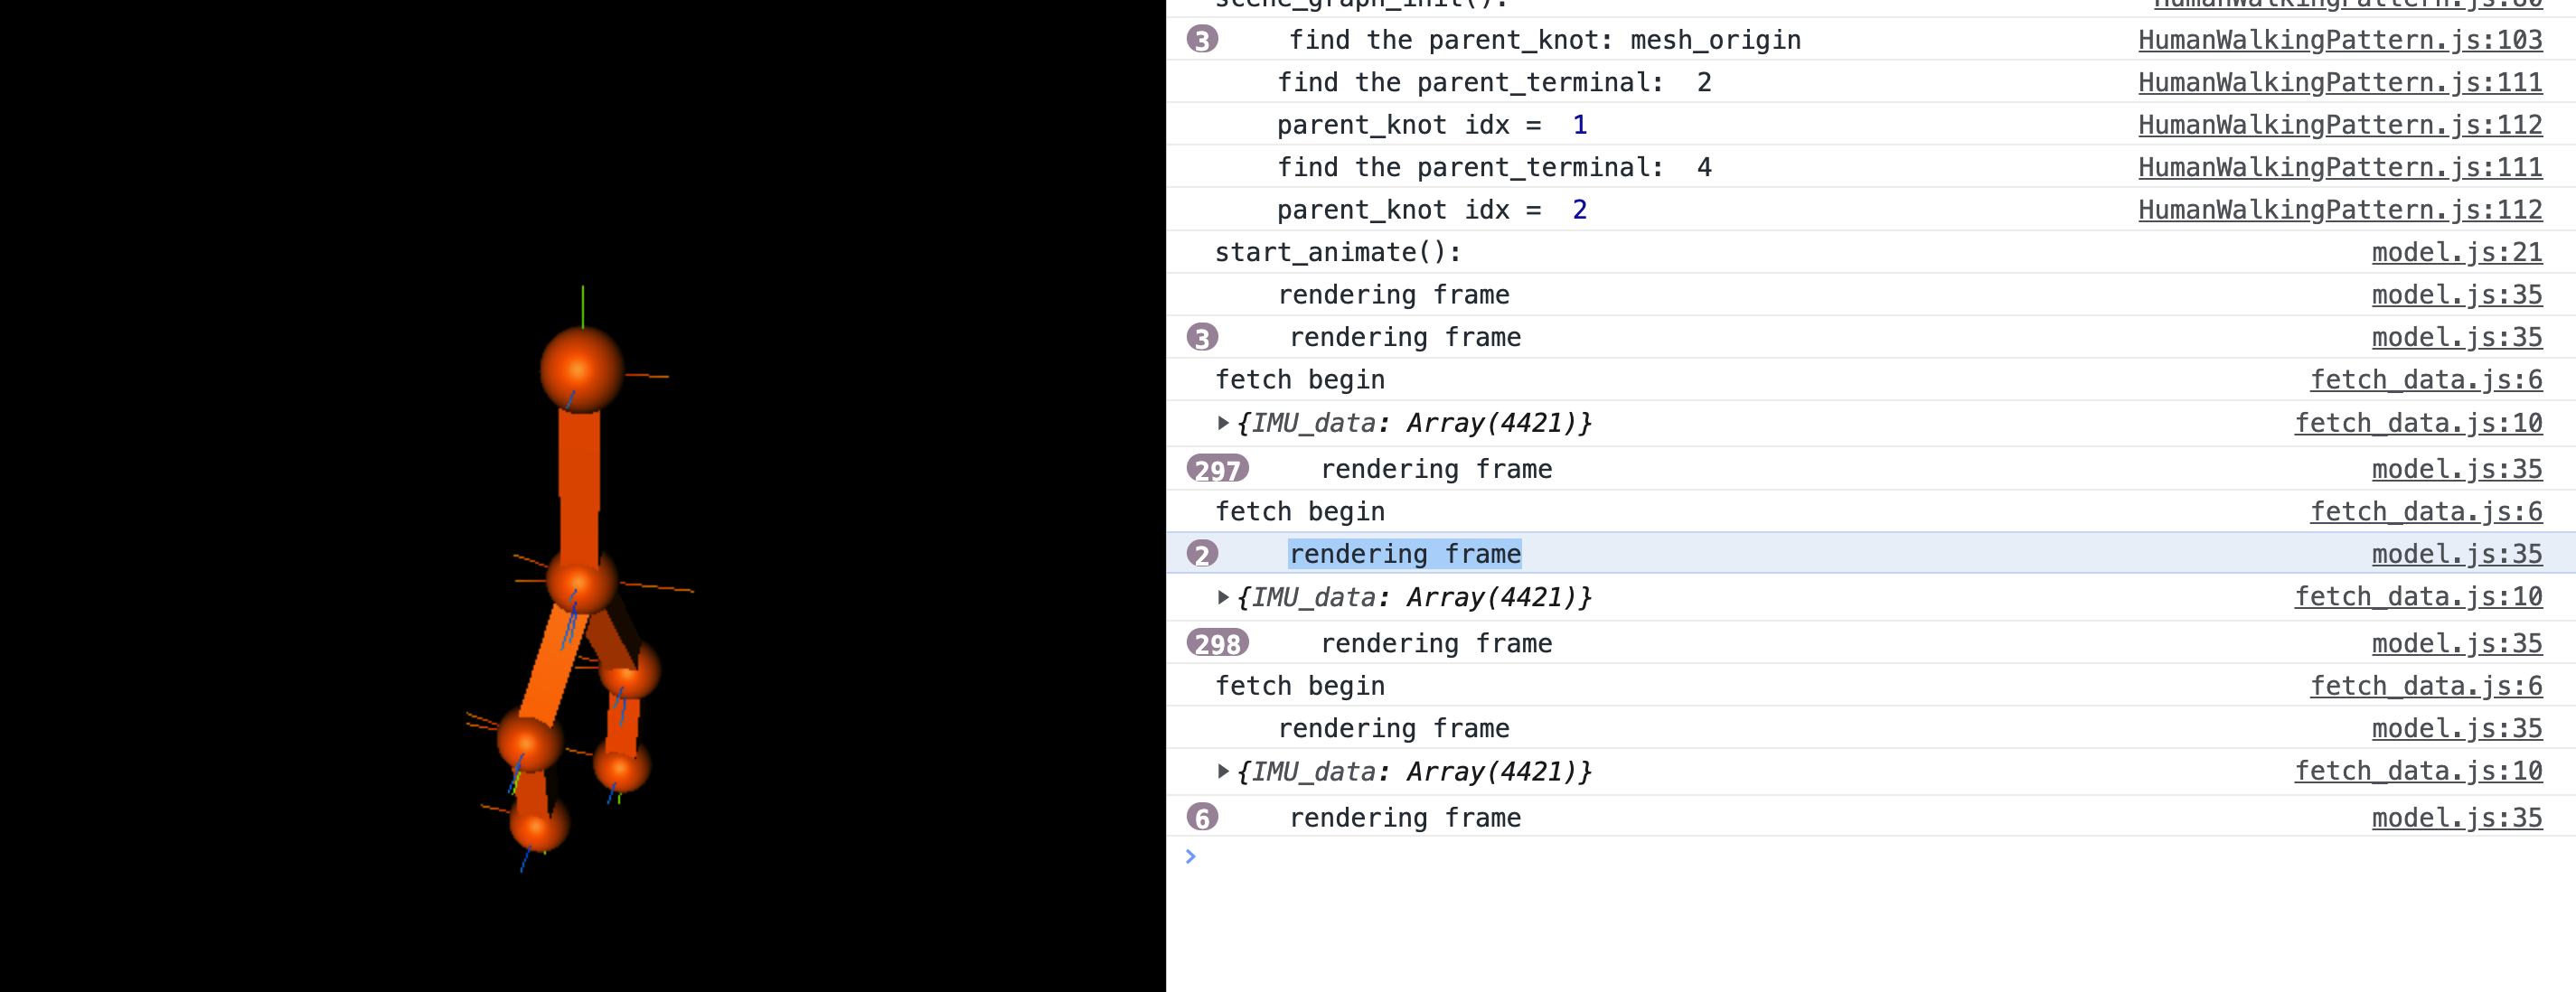
\includegraphics[width=0.9\textwidth]{
		fileForWriting/1mb-test}
	\caption[Time consuming while receiving a single message with a size of 0.73 MB]{Time consuming while fetching a single string message with a size of 0.73 MB. The quantity of poses in such message is 4421.}
	\label{fig:0.73-size}
\end{figure}
%--------End of this FIGURE -----------

By comparison, the thread needed 42 frame intervals to completely hold a 14.4 MB message.

%-----------This is a FIGURE-----------------------
\begin{figure}[htbp]
	\centering
	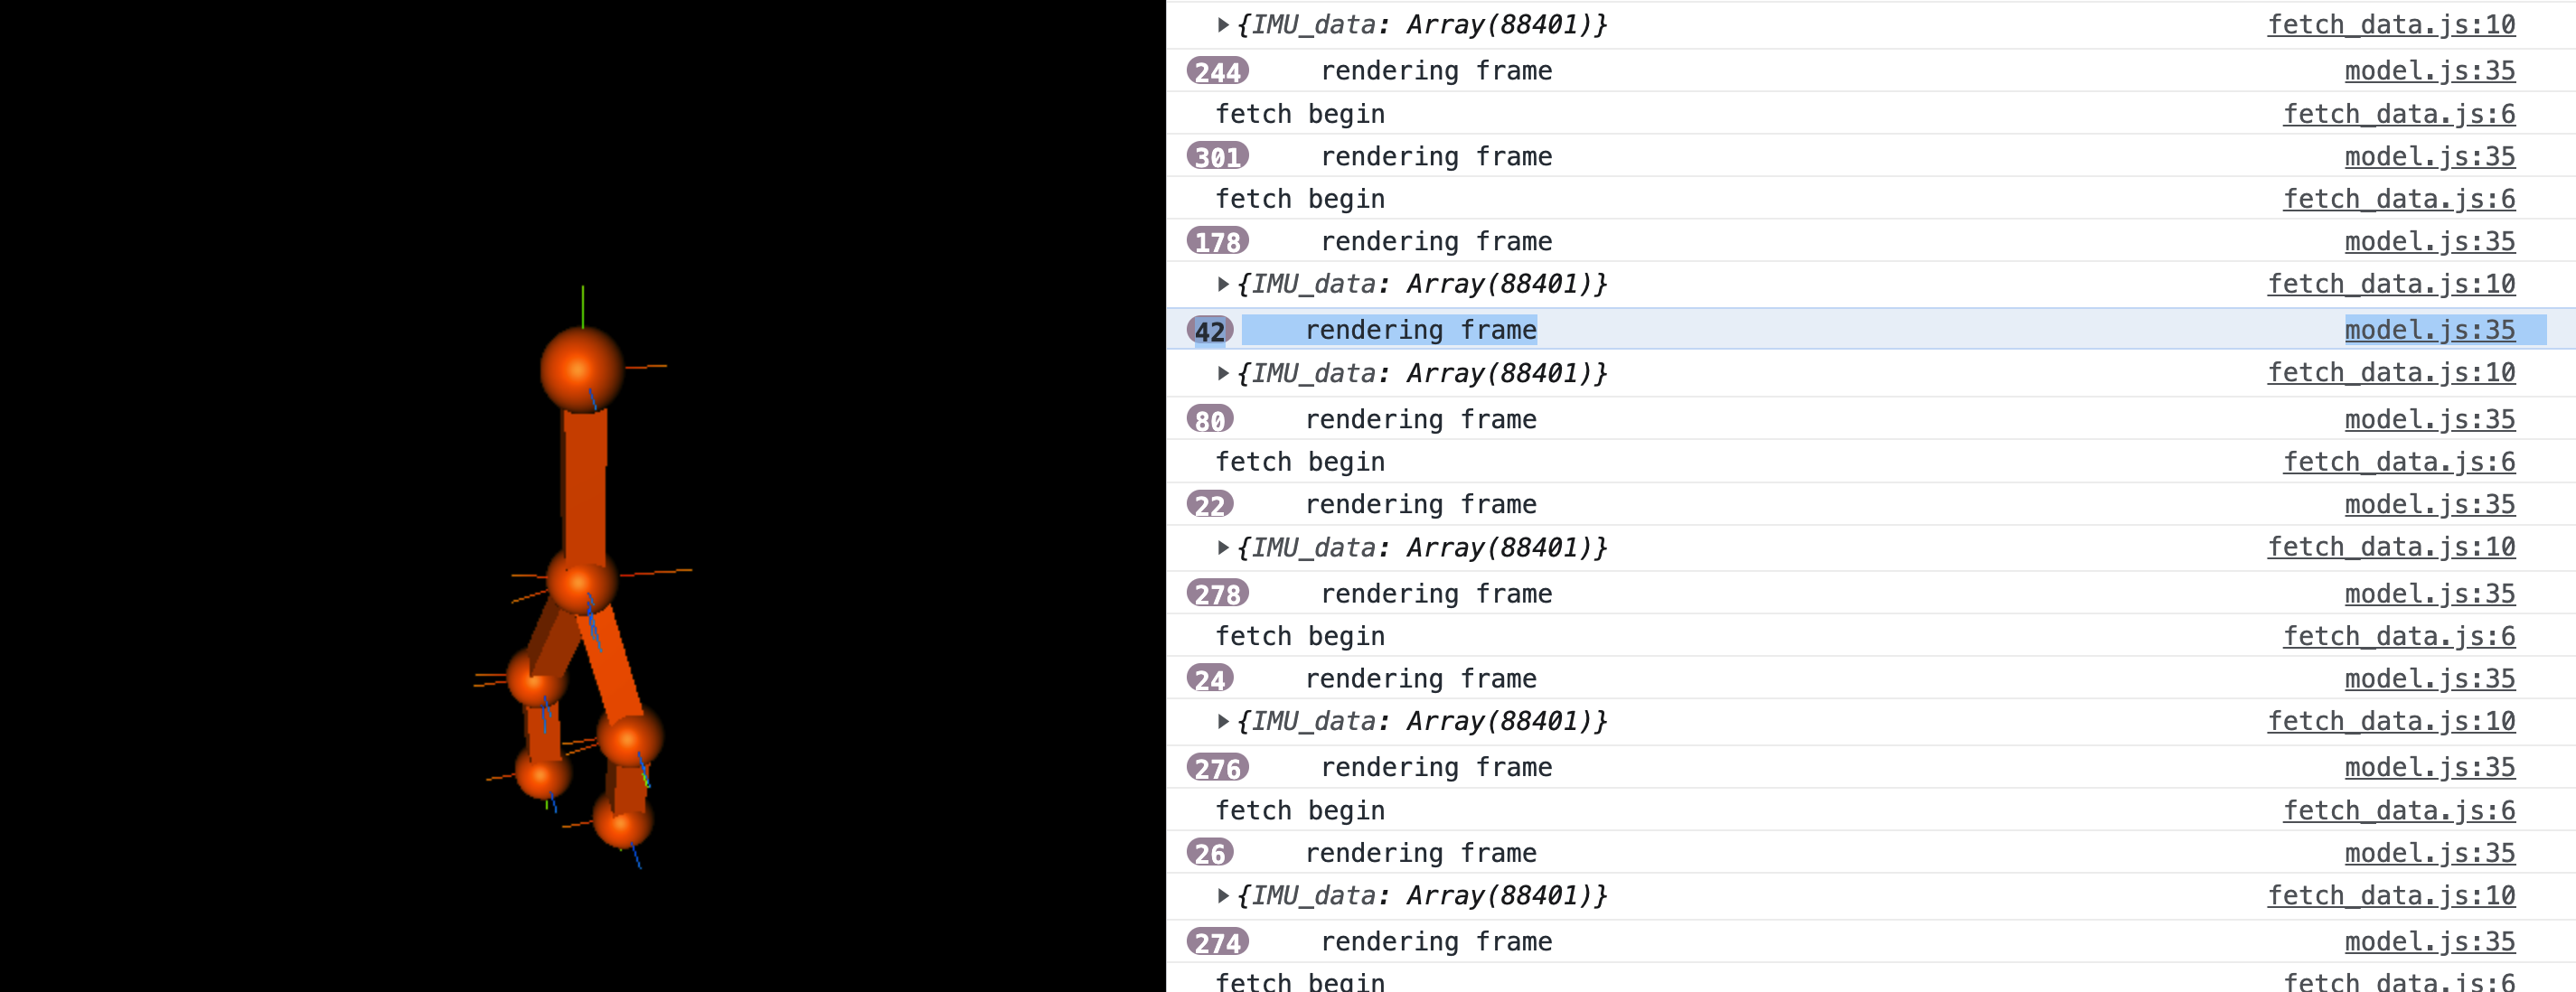
\includegraphics[width=0.9\textwidth]{
		fileForWriting/14mb-test}
	\caption[Time consuming while receiving a single message with a size of 14.4 MB]{Time consuming while fetching a single string message with a size of 14.4 MB. The quantity of poses in such message is 88401.}
	\label{fig:14-size}
\end{figure}
%--------End of this FIGURE -----------

\section{Final Performance}

%-----------This is a FIGURE-----------------------
\begin{figure}[htbp]
	\centering
	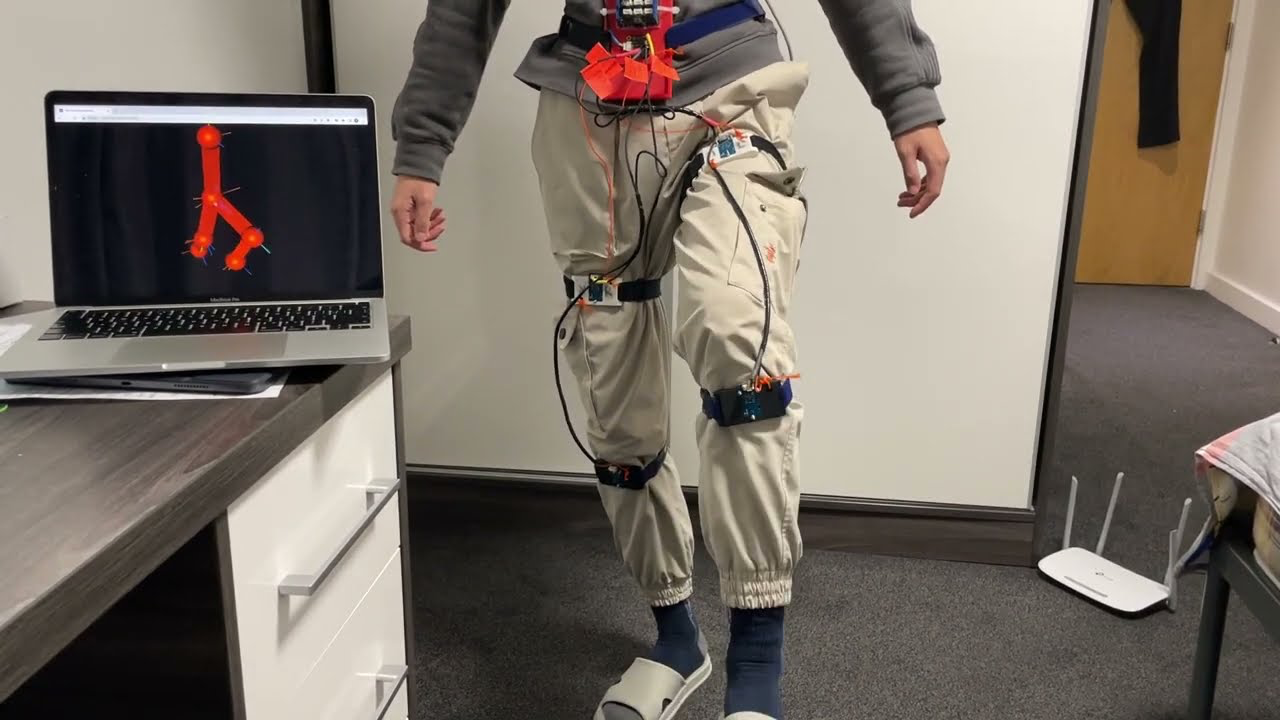
\includegraphics[width=1\textwidth]{
		fileForWriting/youtube-page}
	\caption[A full testing with four IMUs and wireless communication]{A full testing with four IMUs and wireless communication.}
	\label{fig:youtube-demo}
\end{figure}
%--------End of this FIGURE -----------


As presented in the videos at~\cite{youtube-demo},
available via the QR codes in the
footnote\footnote{
\includegraphics[width=1.4cm]{fileForWriting/qrcode-youtube}\cite{youtube-demo}.},
the model generated by the displaying engine in the browser was capable of mimicking human leg movements such as lifting the leg forward or stretching it backward.
As a result, the rotation of the leg could also be recognized and displayed, although it was not well demonstrated in the video.
However, movements of extending the leg to the left or right could not be replicated to the digital twin due to the lack of yaw axis data.

After one-fold interpolation, the animation's frame rate could reach up to 40fps.
However, due to potential factors such as communication delays in wireless transmission, the latency between the digital twin and the actual object is still within the range of human perception, approximately 100 ms by estimation.

In addition to the aforementioned results, the inclusion of the threshold operation has resulted in a reduction of jetting artifacts in the animation to some extent.
However, it was also found that as soon as the distance between the Arduino and the router exceeds two or three meters, there is a significant increase in delay, which eventually leads to the displaying engine getting stuck.


  %latency & problems occured
\chapter{Discussion and Conclusions}


\section{Discussion}
\subsection{Arduino:  Euler angle output}
\subsubsection{Data rate}
The data collection frequency for a single round is only 20 Hz, which seems significantly different from the 100 Hz data rate set for the sensors.
However, it should be noted that we have four sensors, and each sensor works at 100Hz to output data.
In a single round, it would take the MCU longer to collect data from these four sensors, and there is also additional time required for the multiplexer to switch between the circuits.
Therefore, the overall output data frequency for the entire pose, which includes data from all four IMUs, should be normal around 20 FPS\@.

In order to increase the sampling frequency, a simple approach is to attempt upgrading the default data rate of the sensors to 1 kHz. However, this places higher demands on the quality of external IIC communication.
Although shielded wires have been employed to transmit data, the length of the wires has exceeded 50cm, which may already be at the limit for IIC communication.
As the IMU sampling frequency increases, the IIC communication lines may become busier and more susceptible to minor external interference.

\subsubsection{Loss of yaw axis data}

Although there was some instability in the yaw data for some unknown reasons, we were still able to create a digital twin that is capable of replicating the motion of kicking forward and backward using the roll axis data to judge.

Future work should locate and solve this problem, where then the displaying engine could have a full functionality.
If feasible, the sensor should also be upgraded to a more powerful one, which may include a temperature compensation circuit to avoid the effect from changing temperature.

\subsection{Displaying engine: flexible configuration}

The result in section~\ref{sec:flexible} indicates that the current displaying engine is sufficient to meet various requirements of modelling, merely generating corresponding skeletons composed of various joints.

However, it is now still difficult to handle an incorrect input.
Once the setting is wrong, the program will fail immediately, without giving any guidelines for the user to diagnose their wrong inputs.
Hence, this could also be a future improvement.


\subsection{Displaying  engine:  asynchronously  fetching data}
With the results in section~\ref{sec:async}, the operation of multi-thread should be particularly useful while sending a large message, at least containing 10,000 poses in single message.
However, in current project, given that the pose data rate was only 20Hz, the quantity in a one message would not exceed 20 poses, or the latency will be at least 1 second.
As a result, the current design of multi-thread has not fully realized its intended function as the size of message is small.

\subsection{Final Performance}

\subsubsection{Latency}
Despite efforts to reduce latency in the current real-time rendering process, such as using message abbreviations and implementing multi-threading for data sending and receiving, further improvements can be made.
One potential solution for the future is to conduct a thorough analysis of the latency from the Arduino to the display engine.
This analysis can help identify the primary sources of delay, allowing for targeted improvements.

\subsubsection{Adaptation}
The current device is lightweight and suitable for use by humans, but it is not compatible with birds.
Therefore, to collect motion data of birds in outdoor settings in the future, a complete redesign of the data collection layer is necessary.
For instance, the smaller Arduino Nano Every board can be utilized, and new wearable solutions can be explored, taking inspiration from the structure of birds themselves.
However, some other parts, such as the displaying engine, only require partial improvements as they have already been designed to generate corresponding models flexibly with input text.

\subsubsection{Accuracy}
Although accuracy was not listed as one of the main objectives for current project, it may be a key focus for future work, especially when it comes to precisely mirroring complex motions.
This could become particularly important when the device is applied to study the flight dynamics of birds, where accurate data is essential.

For instance, in the case of studying bird flight, the device will need to capture and analyze a vast amount of data with high accuracy in order to gain insights into the complex mechanics of avian flight.
By achieving a higher level of accuracy in motion tracking, researchers can better understand the nuances of bird flight, including the subtle changes in wing angle, speed, and other factors that can affect flight performance.
This can ultimately lead to a better understanding of the biomechanics of avian flight and help researchers design better drones and other aircraft.




\section{Conclusions}
\parindent

In summary, this research project managed to create a non-optical bio-logging system that utilizes four IMUs to capture motion data for human objects.
Moreover, the system includes wireless communication and a displaying engine that creates a digital twin of the human lower body in the browser.
This digital representation can mimic real leg movements such as lifting the leg forward or stretching it backward, with an acceptable latency.
Given the flexibility of the system, it also has the potential to be further enhanced to investigate avian flight dynamics or other zoology-related topics.






\singlespace
\bibliographystyle{IEEEtran}
\bibliography{/Users/shenyixiao/Repo/Final-Report/src/MyRefs}
\addcontentsline{toc}{chapter}{References} % to add it to the table of contents

%appendix
\newpage
\appendix
\appendixpage
\addappheadtotoc

\chapter{Project Management Forms}
%Appendix A: Attach the project management forms (Role allocation/responsibility matrix, Contribution to project deliverables, Attendance record, Supervisor weekly meeting log) to your project report as an appendix. Other supporting documents you may have used such as personal notes/notebooks/logbooks should not be included in the report.


%-----------This is a FIGURE-----------------------
\begin{figure}[htbp]
	\centering
	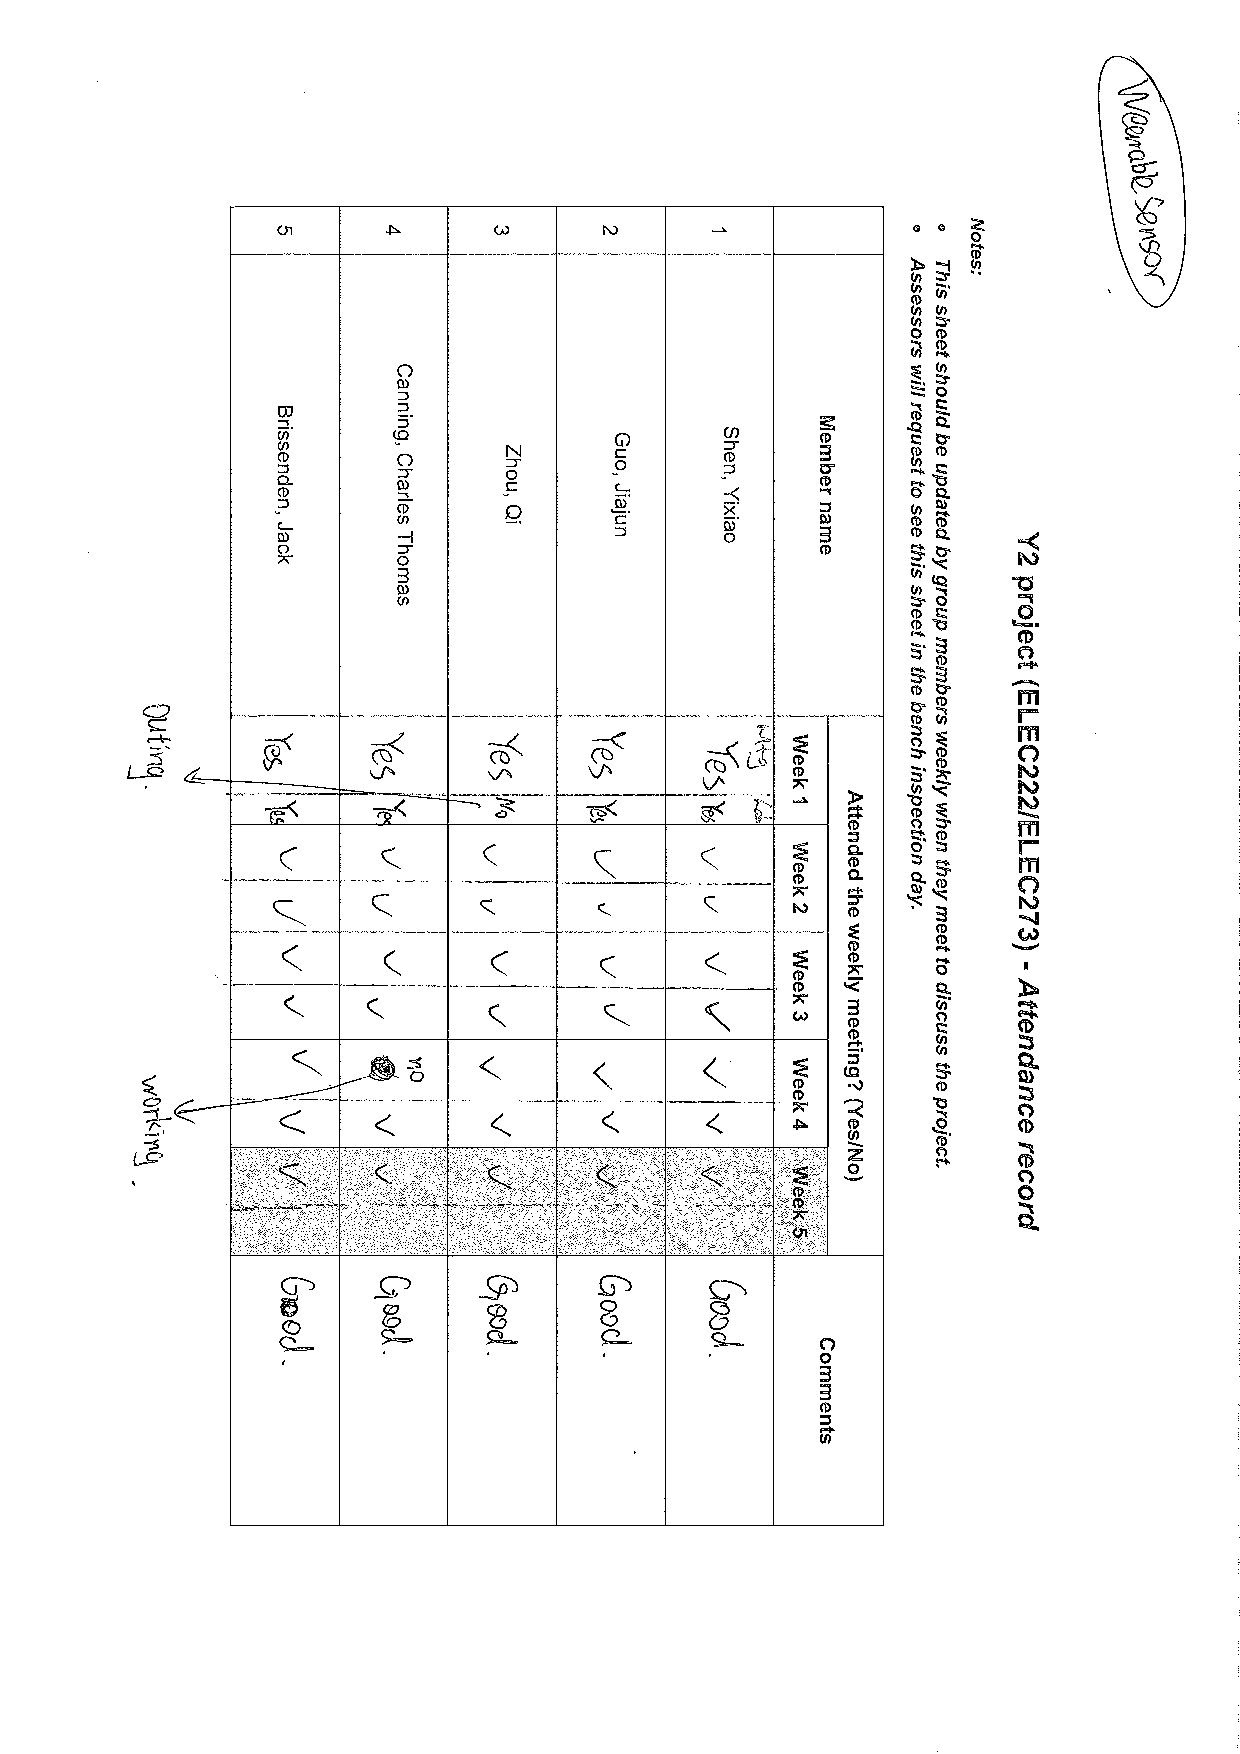
\includegraphics[width=\textwidth]{
		appendix/attendence-record}
	\caption{Attendence record.}
	\label{fig:attendence-record}
\end{figure}
%--------End of this FIGURE -----------
%-----------This is a FIGURE-----------------------
\begin{figure}[htbp]
	\centering
	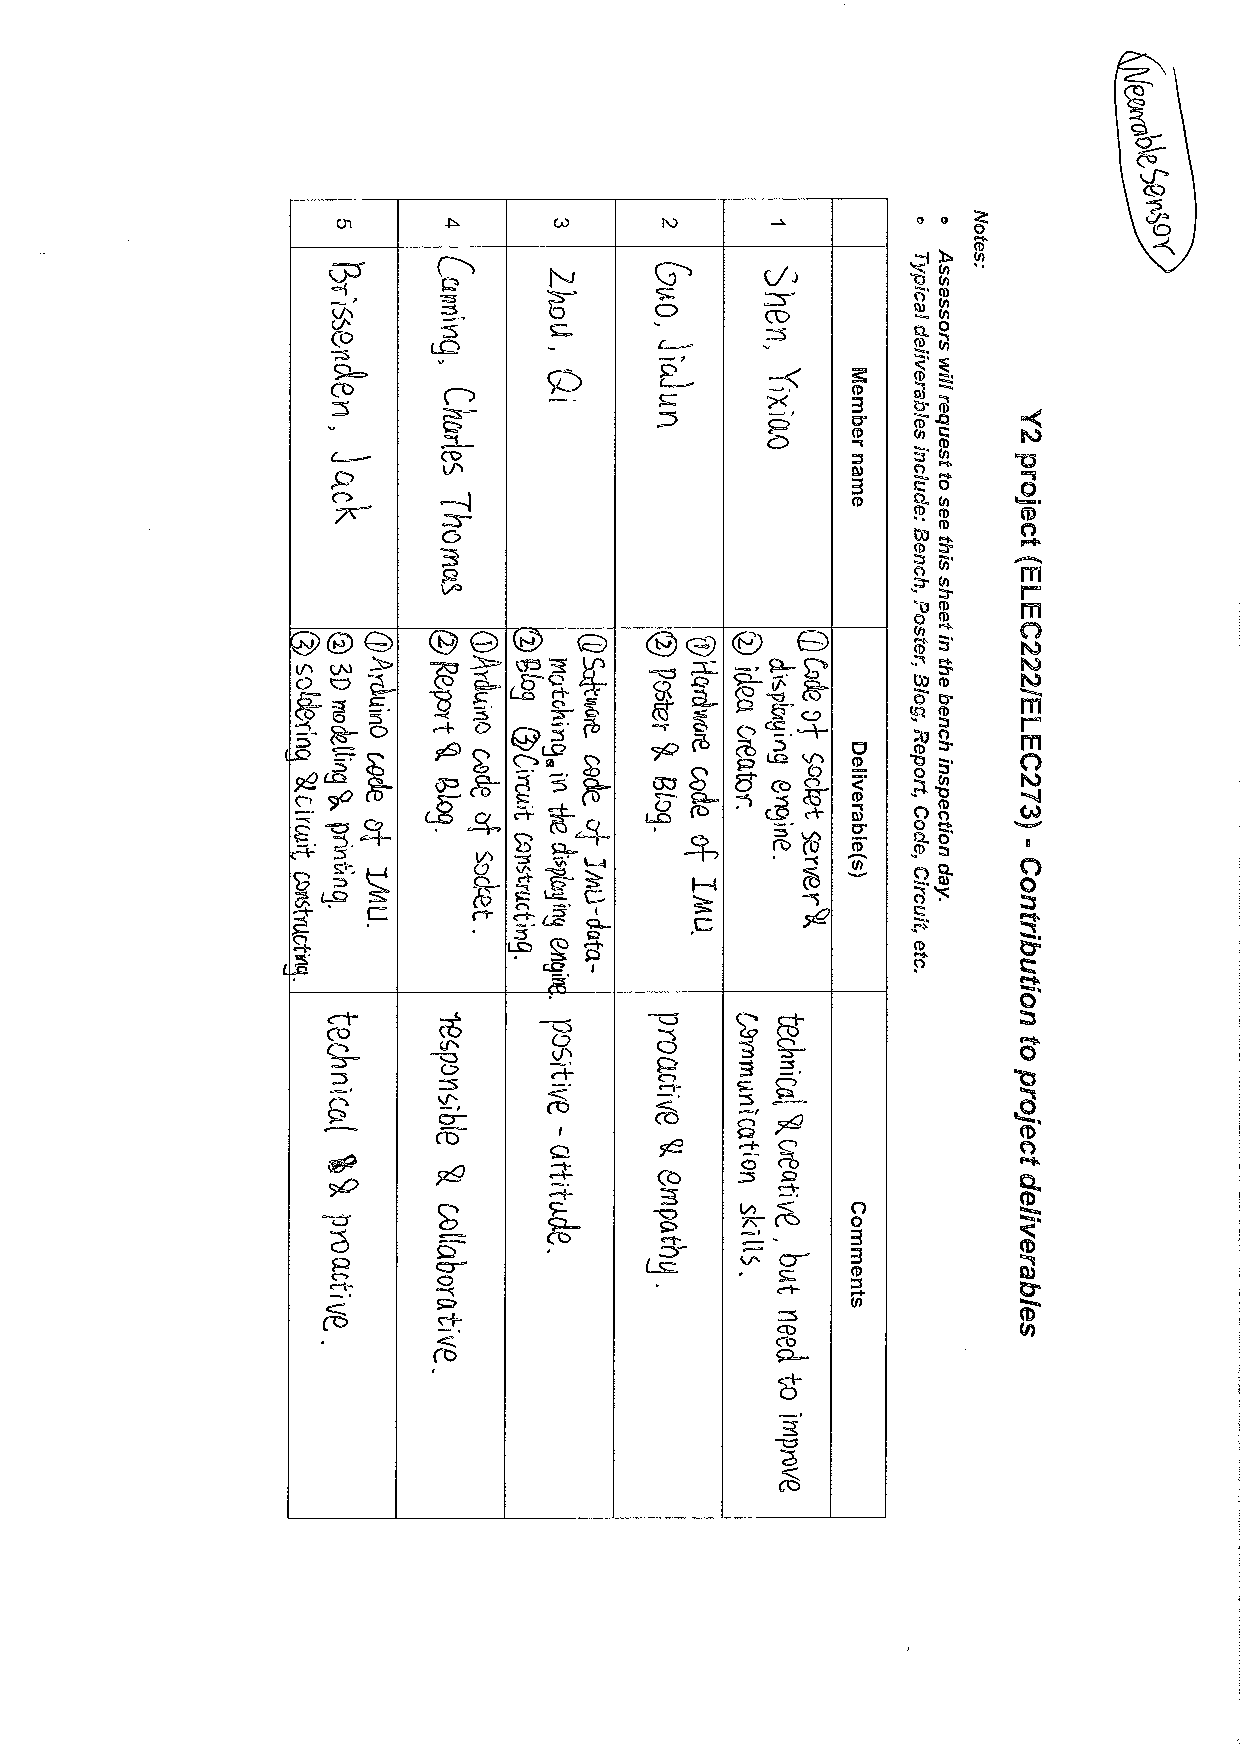
\includegraphics[width=\textwidth]{
		appendix/project-contribution}
	\caption{Contribution to project deliverables.}
	\label{fig:project-contribution}
\end{figure}
%--------End of this FIGURE -----------
%-----------This is a FIGURE-----------------------
\begin{figure}[htbp]
	\centering
	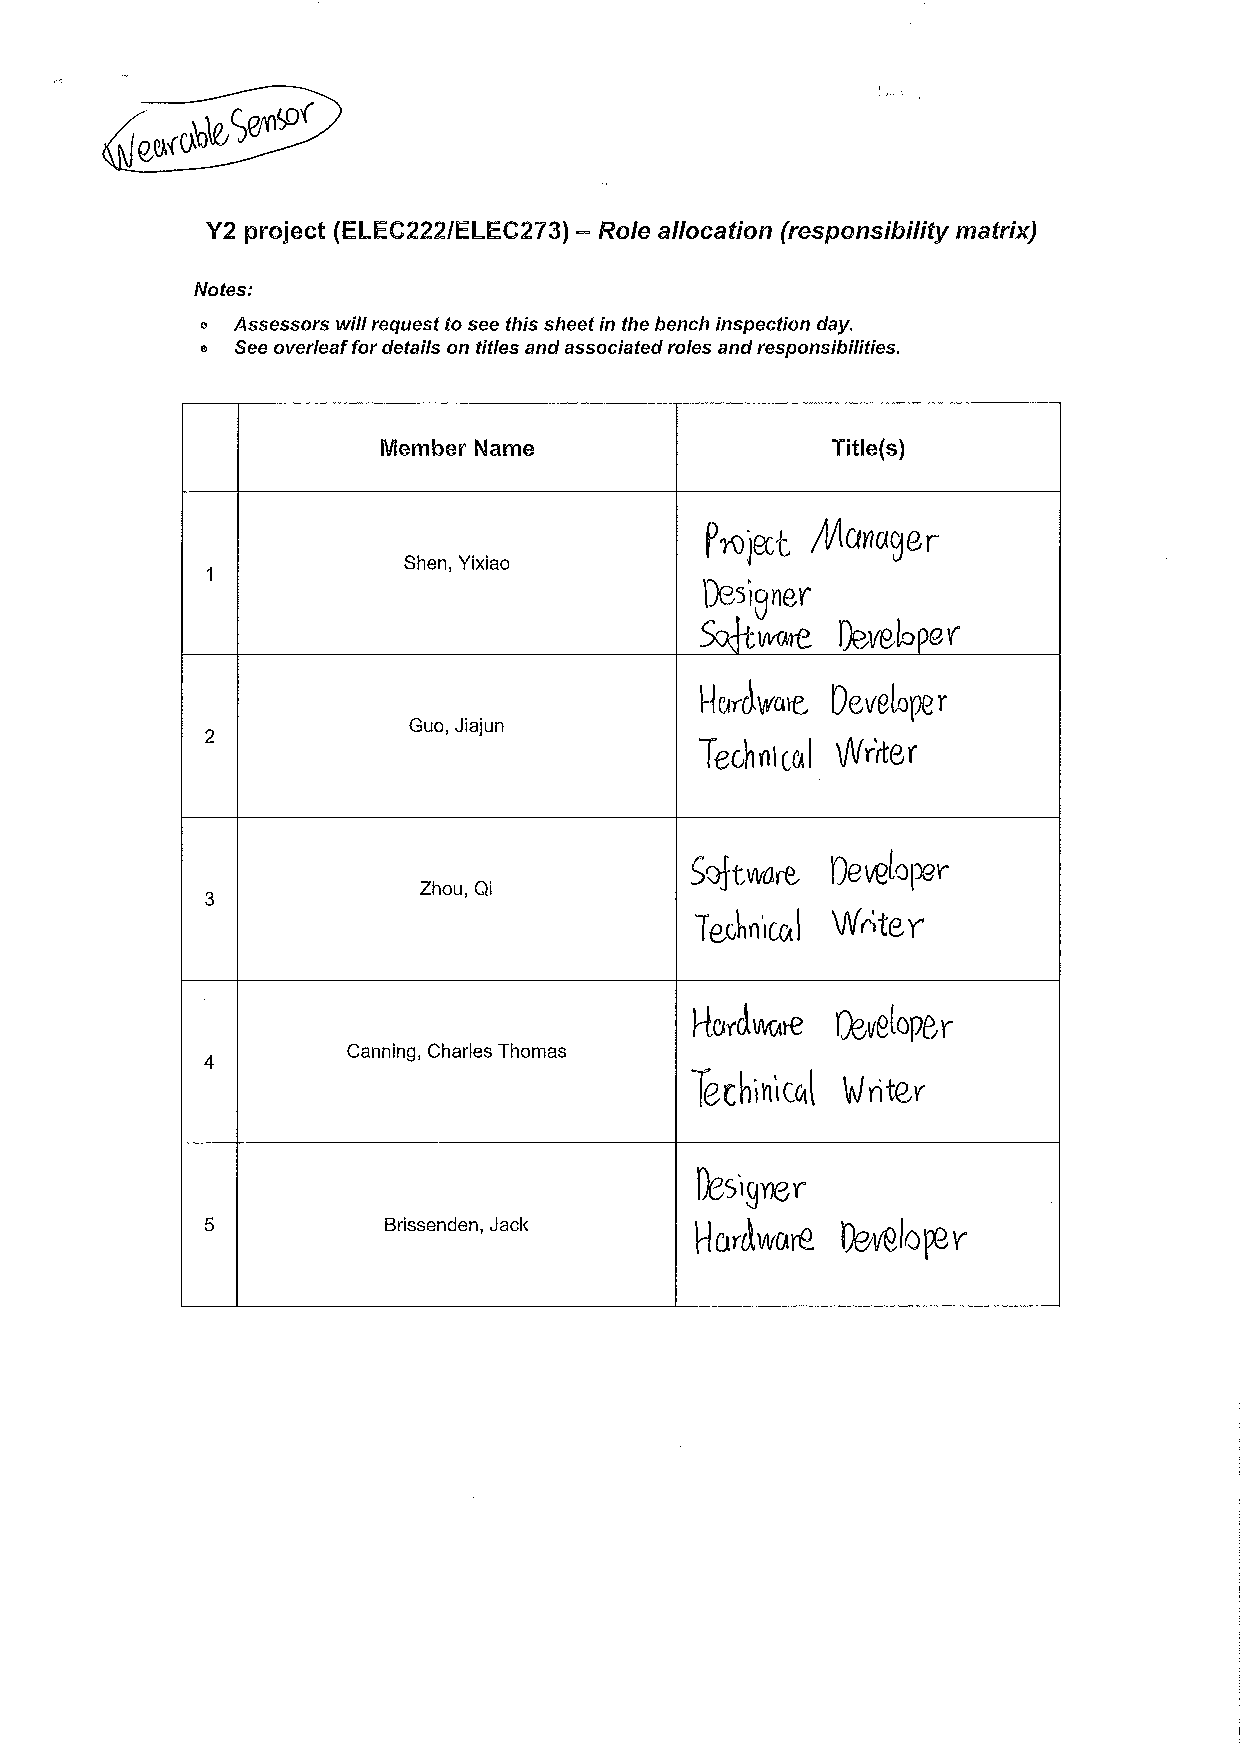
\includegraphics[width=\textwidth]{
		appendix/role-allocation}
	\caption{Role allocation (responsibility matrix).}
	\label{fig:role-allocation}
\end{figure}
%--------End of this FIGURE -----------

%-----------This is a FIGURE-----------------------
\begin{figure}[htbp]
	\centering
	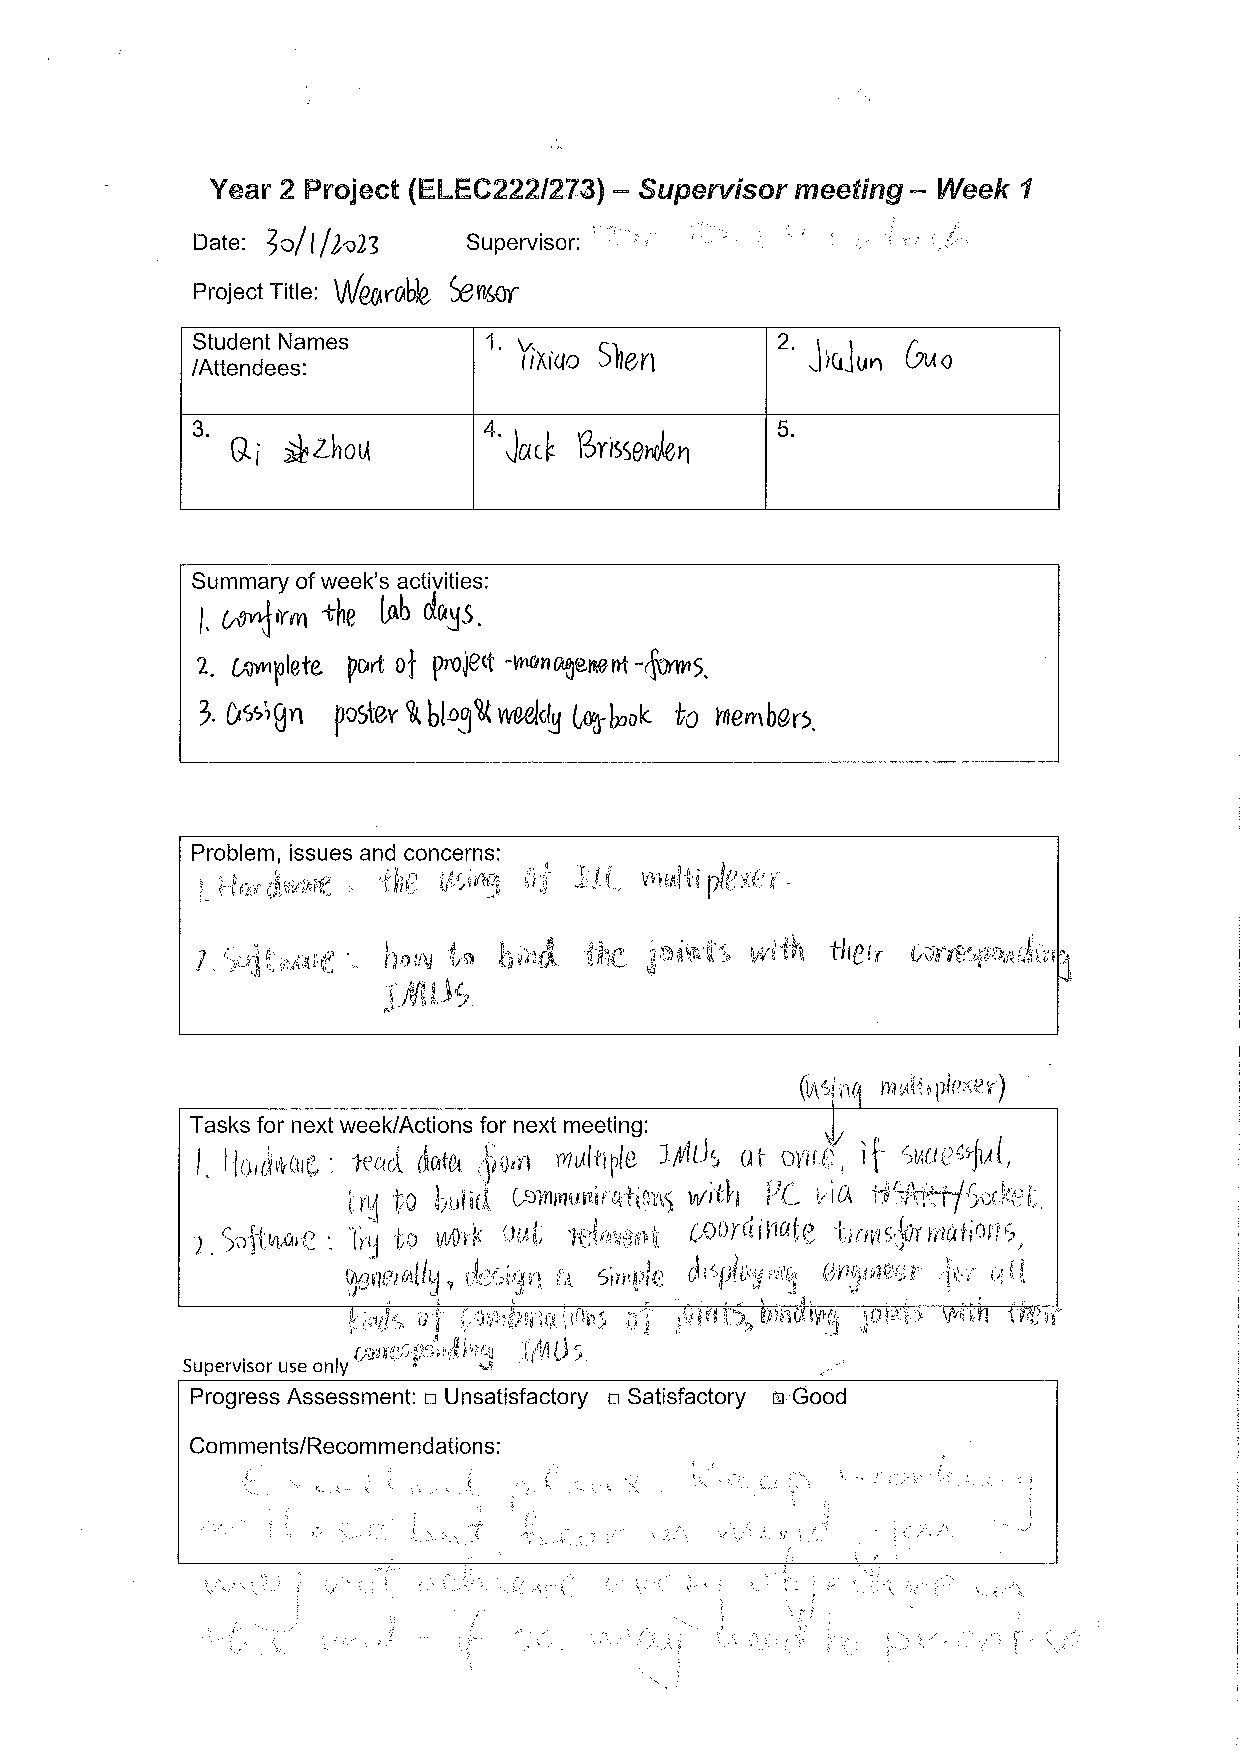
\includegraphics[width=\textwidth]{
		appendix/meeting-log-1}
	\caption{Supervisor weekly meeting log 1.}
	\label{fig:meeting-log-1}
\end{figure}
%--------End of this FIGURE -----------
%-----------This is a FIGURE-----------------------
\begin{figure}[htbp]
	\centering
	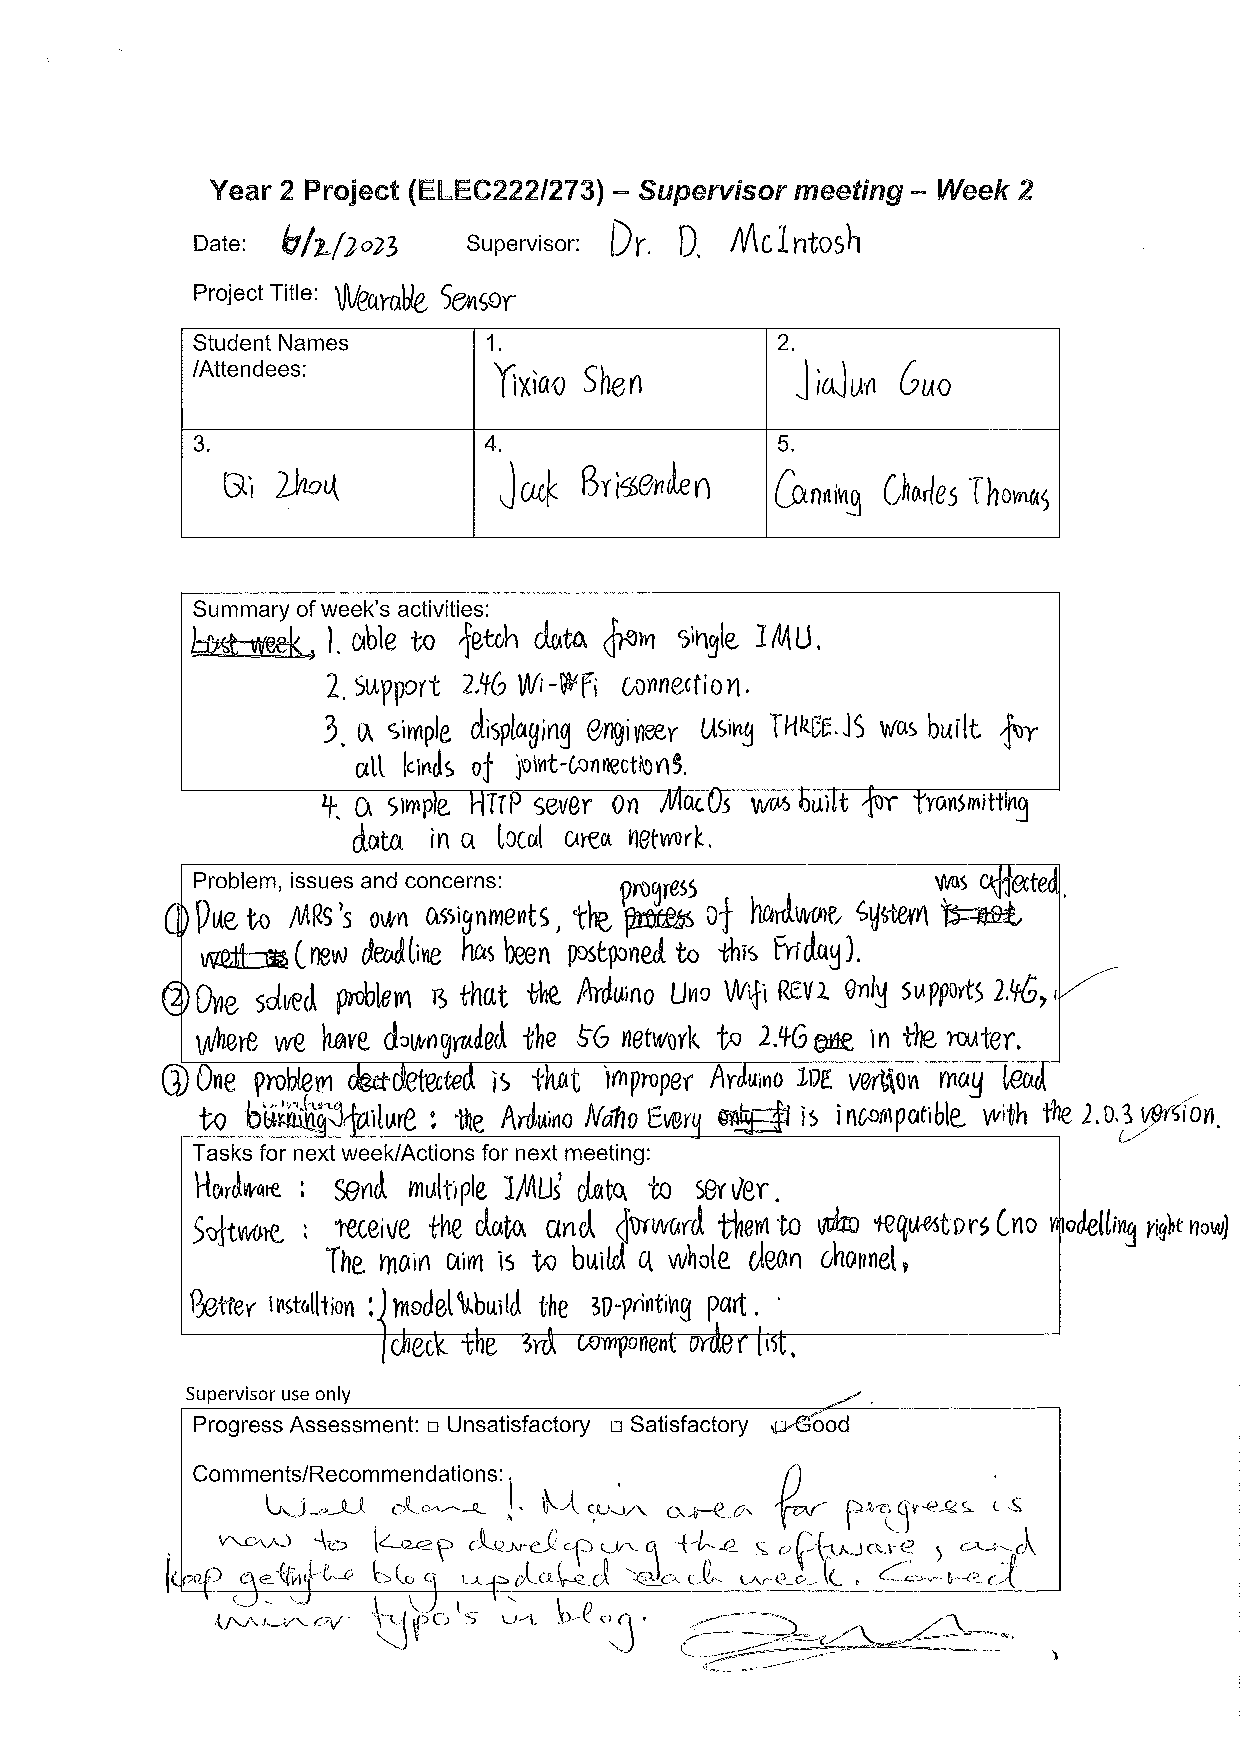
\includegraphics[width=\textwidth]{
		appendix/meeting-log-2}
	\caption{Supervisor weekly meeting log 2.}
	\label{fig:meeting-log-2}
\end{figure}
%--------End of this FIGURE -----------
%-----------This is a FIGURE-----------------------
\begin{figure}[htbp]
	\centering
	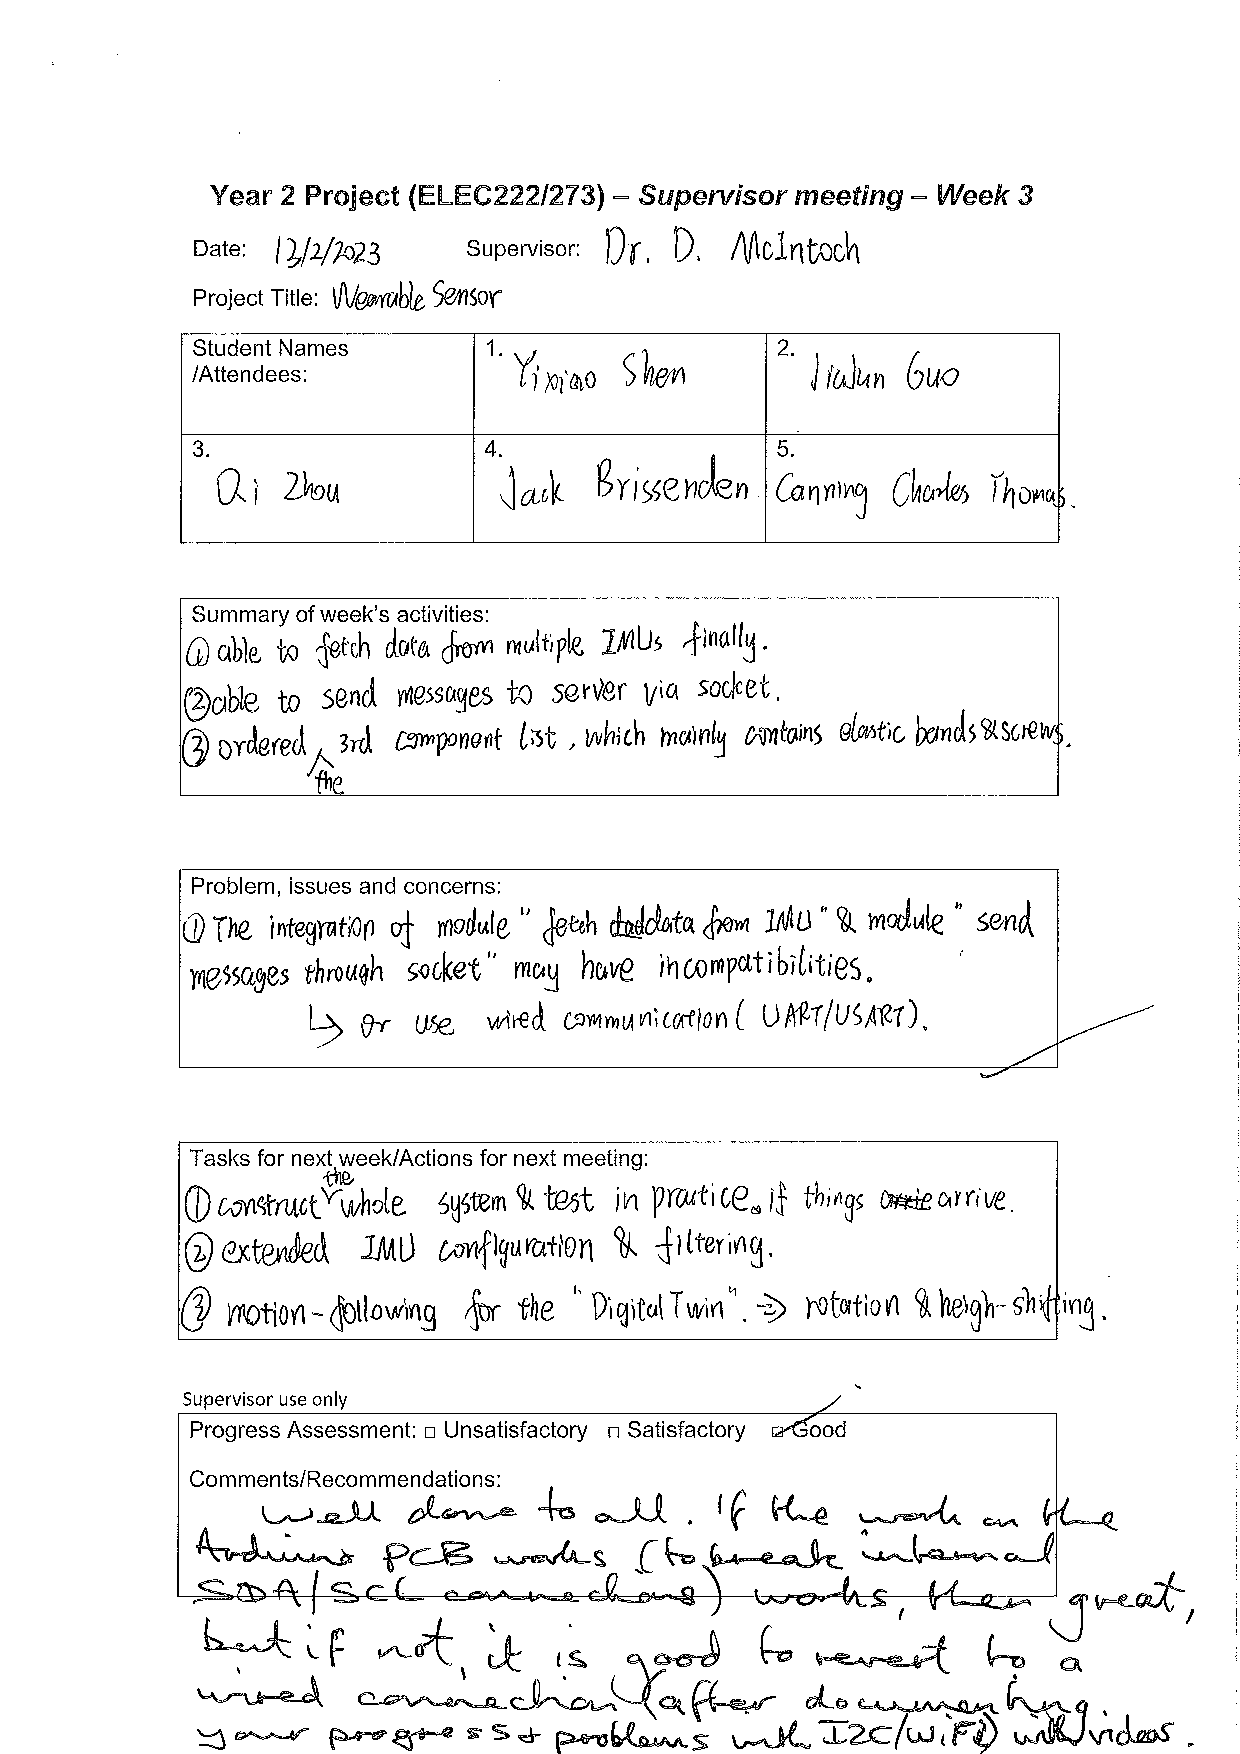
\includegraphics[width=\textwidth]{
		appendix/meeting-log-3}
	\caption{Supervisor weekly meeting log 3.}
	\label{fig:meeting-log-3}
\end{figure}
%--------End of this FIGURE -----------
%-----------This is a FIGURE-----------------------
\begin{figure}[htbp]
	\centering
	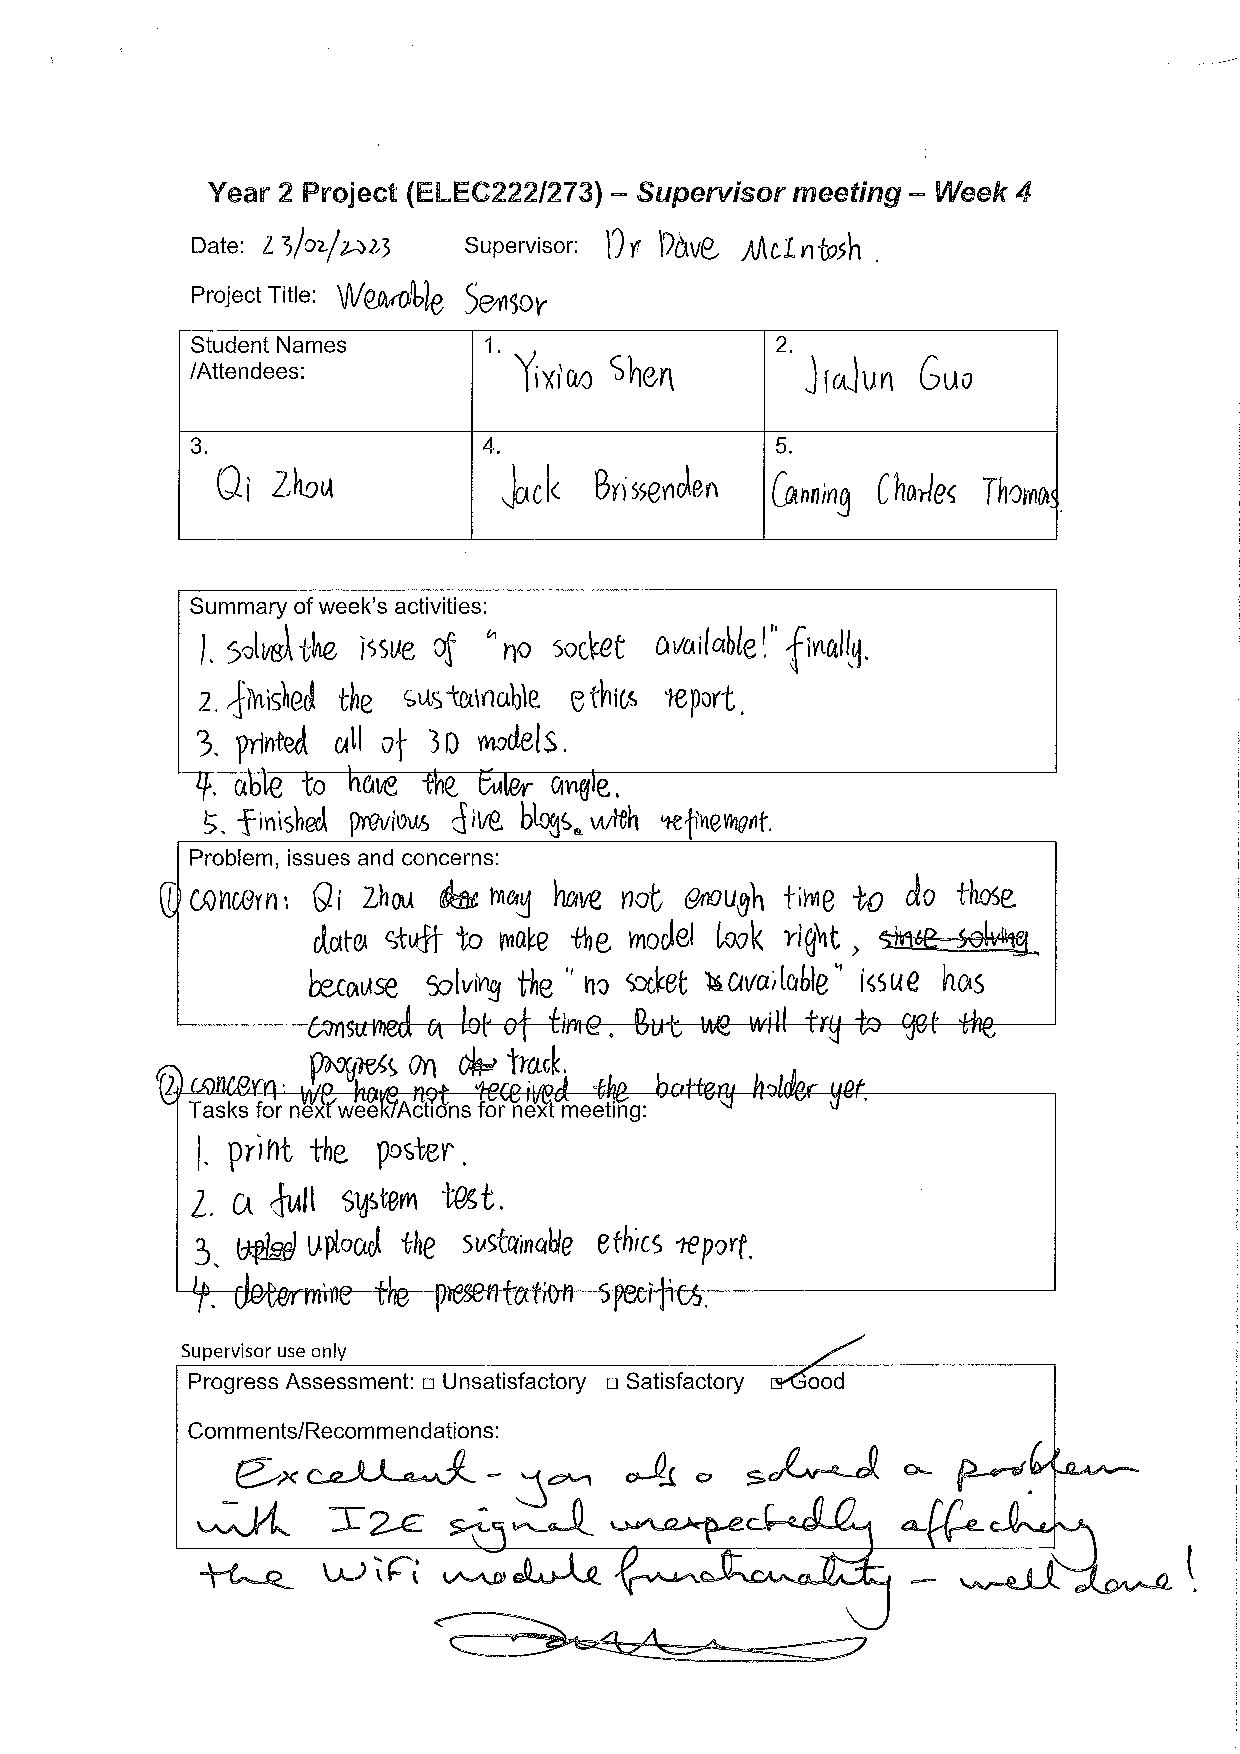
\includegraphics[width=\textwidth]{
		appendix/meeting-log-4}
	\caption{Supervisor weekly meeting log 4.}
	\label{fig:meeting-log-4}
\end{figure}
%--------End of this FIGURE -----------



\chapter{A Breakdown of Individual Contributions}

%-----------This is a FIGURE-----------------------
\begin{figure}[htbp]
	\centering              %=left botm right top
	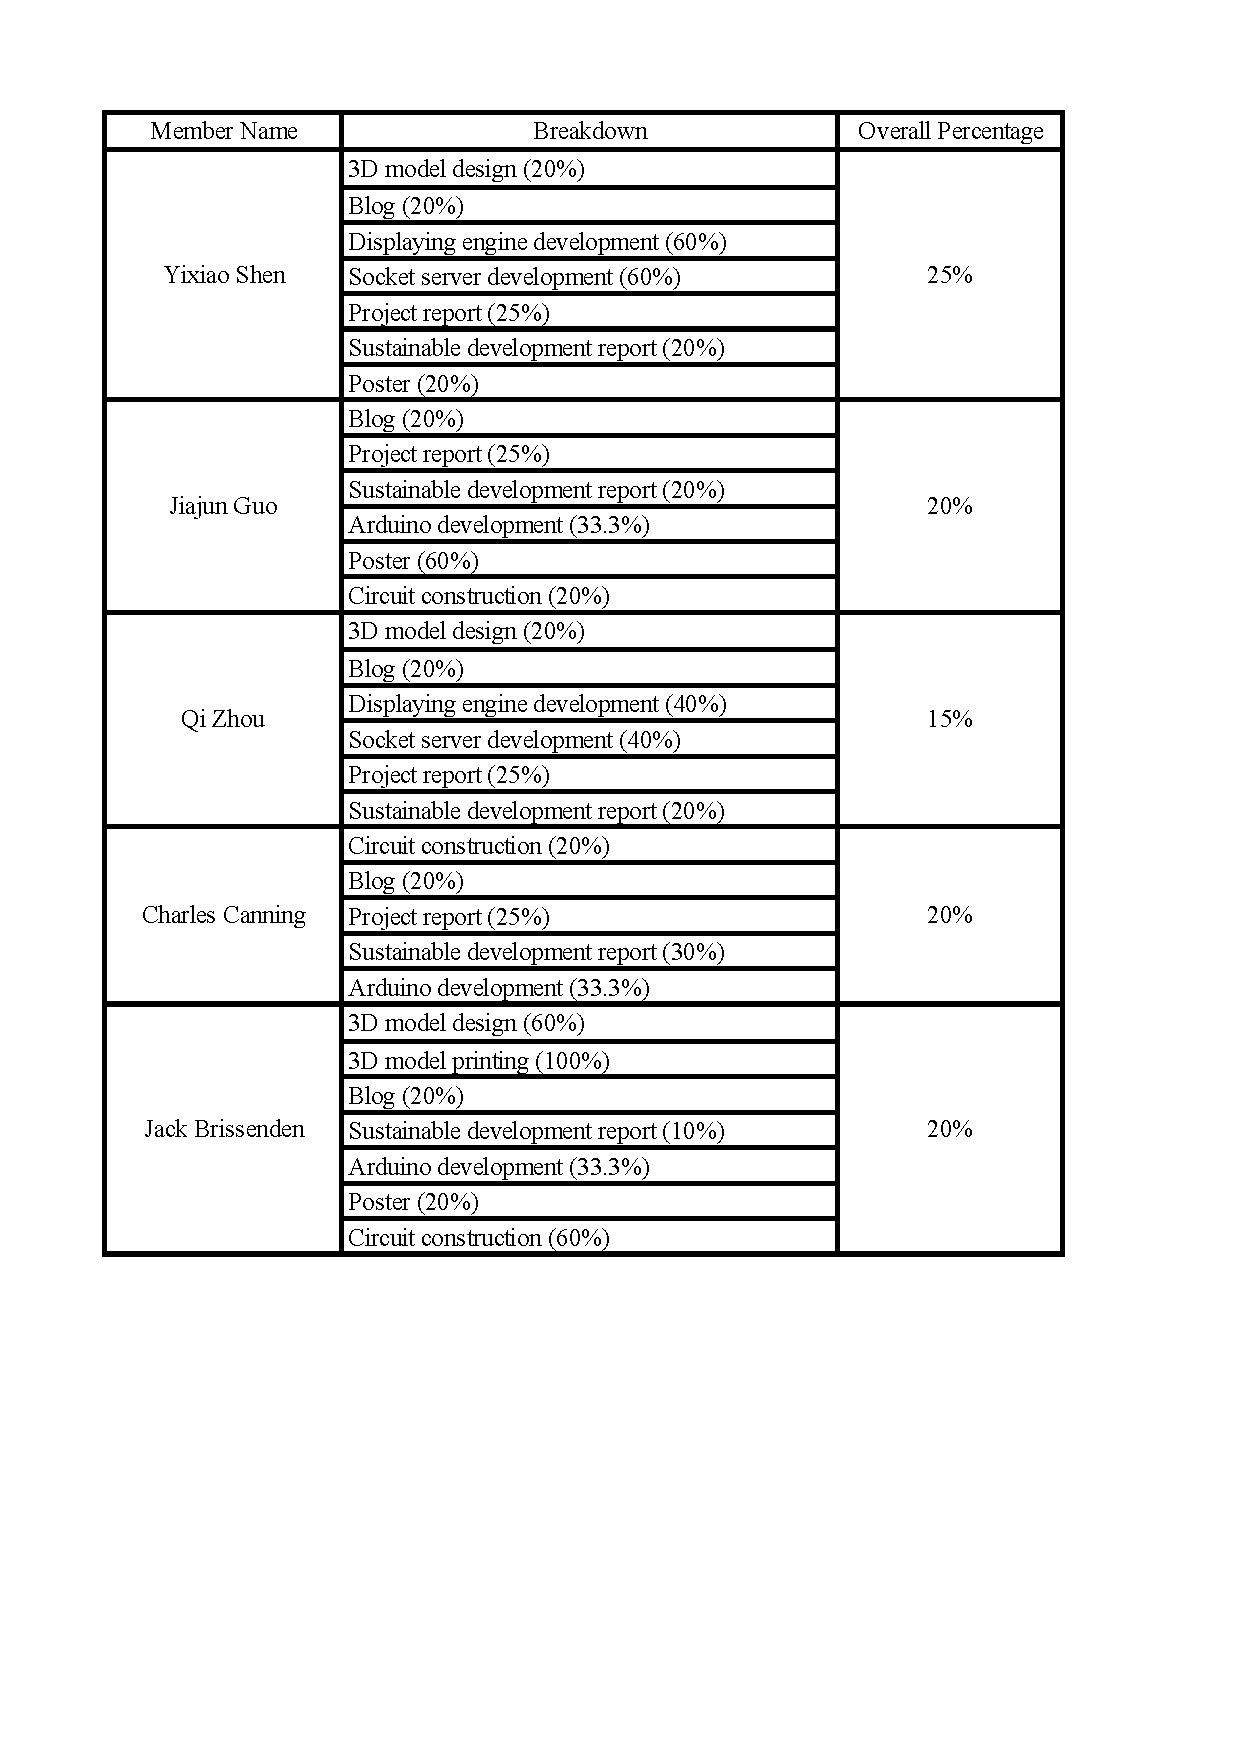
\includegraphics[clip, trim=1.5cm 8cm 1.5cm 1.5cm, width=\textwidth]{
		appendix/breakdown}
	\caption[Breakdown of individual contributions]{Breakdown of individual contributions.}
	\label{fig:breakdown}
\end{figure}
%--------End of this FIGURE -----------




\chapter{Datasheets}

%-----------This is a FIGURE-----------------------
\begin{figure}[htbp]
	\centering
	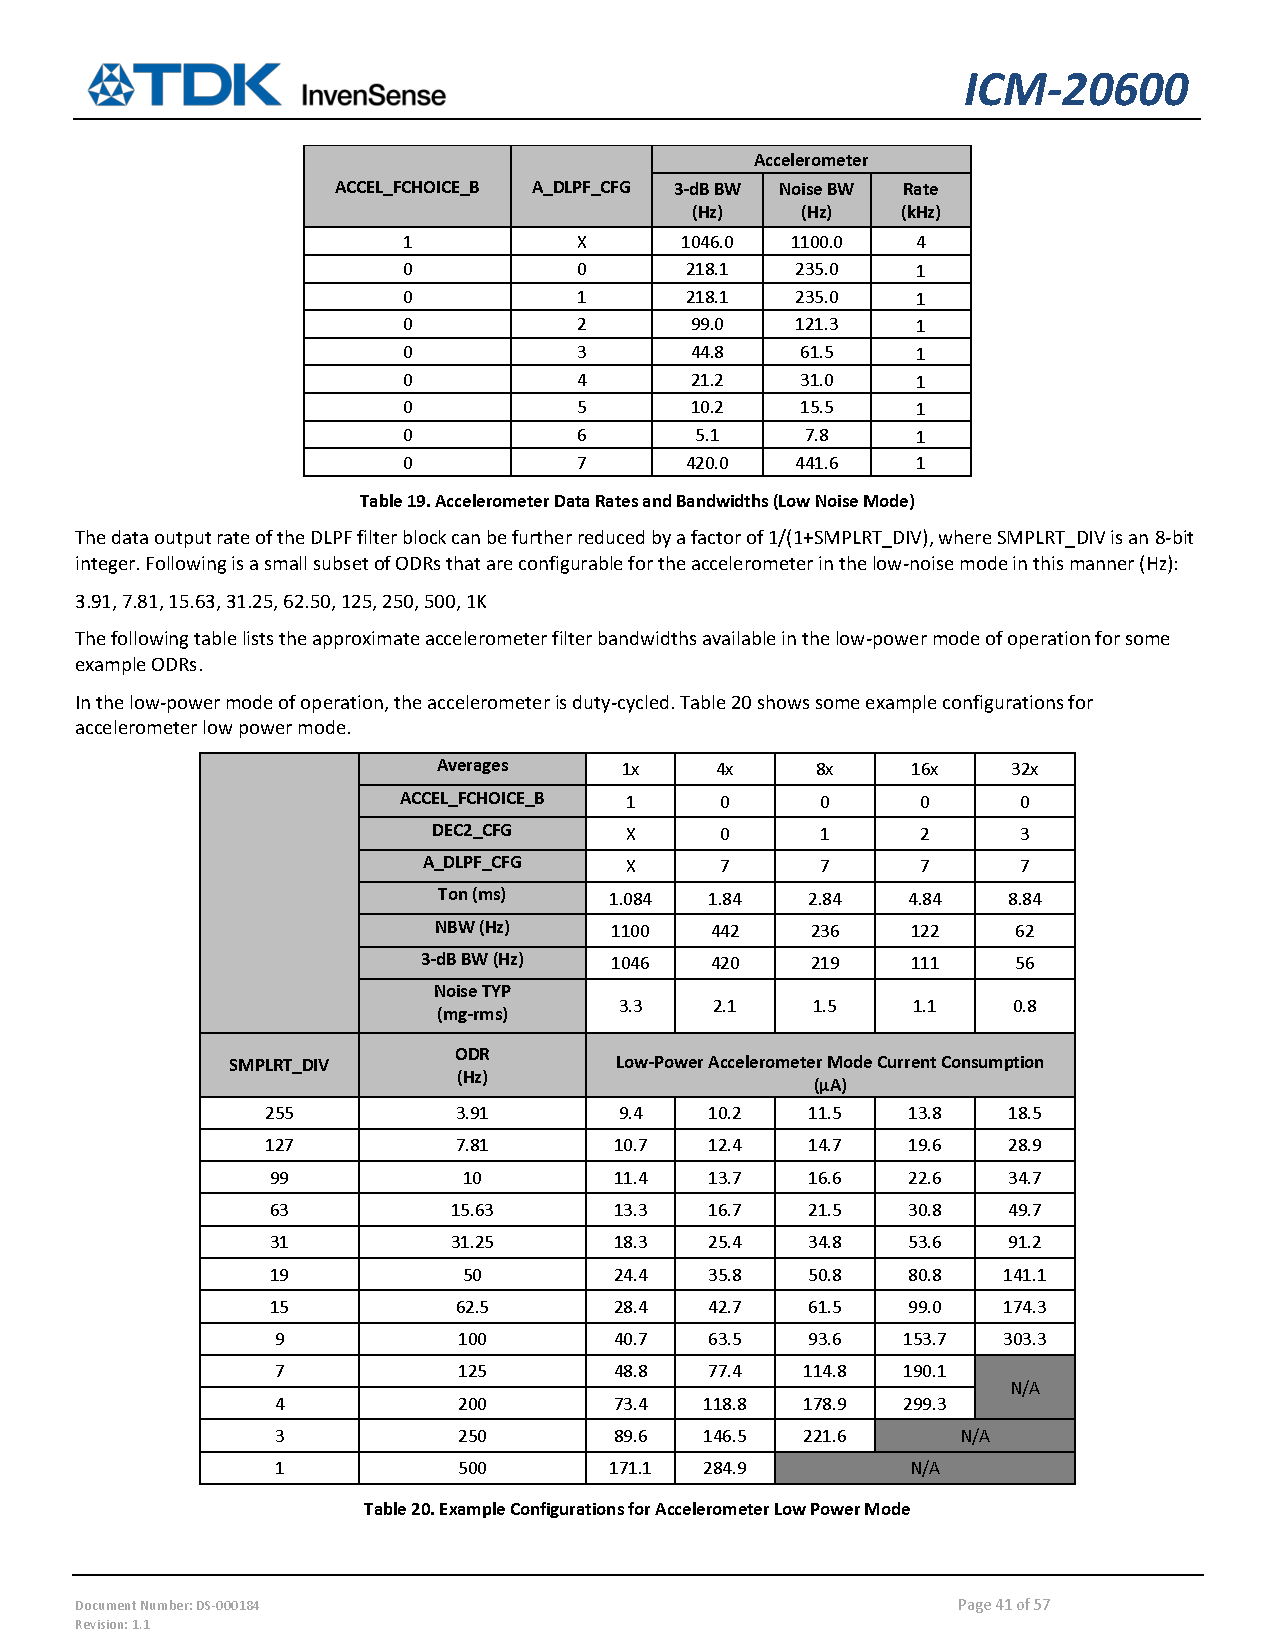
\includegraphics[width=1.1\textwidth]{
		fileForWriting/data rate seeting}
	\caption[Datasheet of the ICM20600 sensor component.]{Example output data rateconfigurations for accelerometer in low power mode, from datasheet~\cite{invensense-icm20600-datasheet}.}
	\label{fig:data-rate-config}
\end{figure}
%--------End of this FIGURE -----------

%-----------This is a FIGURE-----------------------
\begin{figure}[htbp]
	\centering
	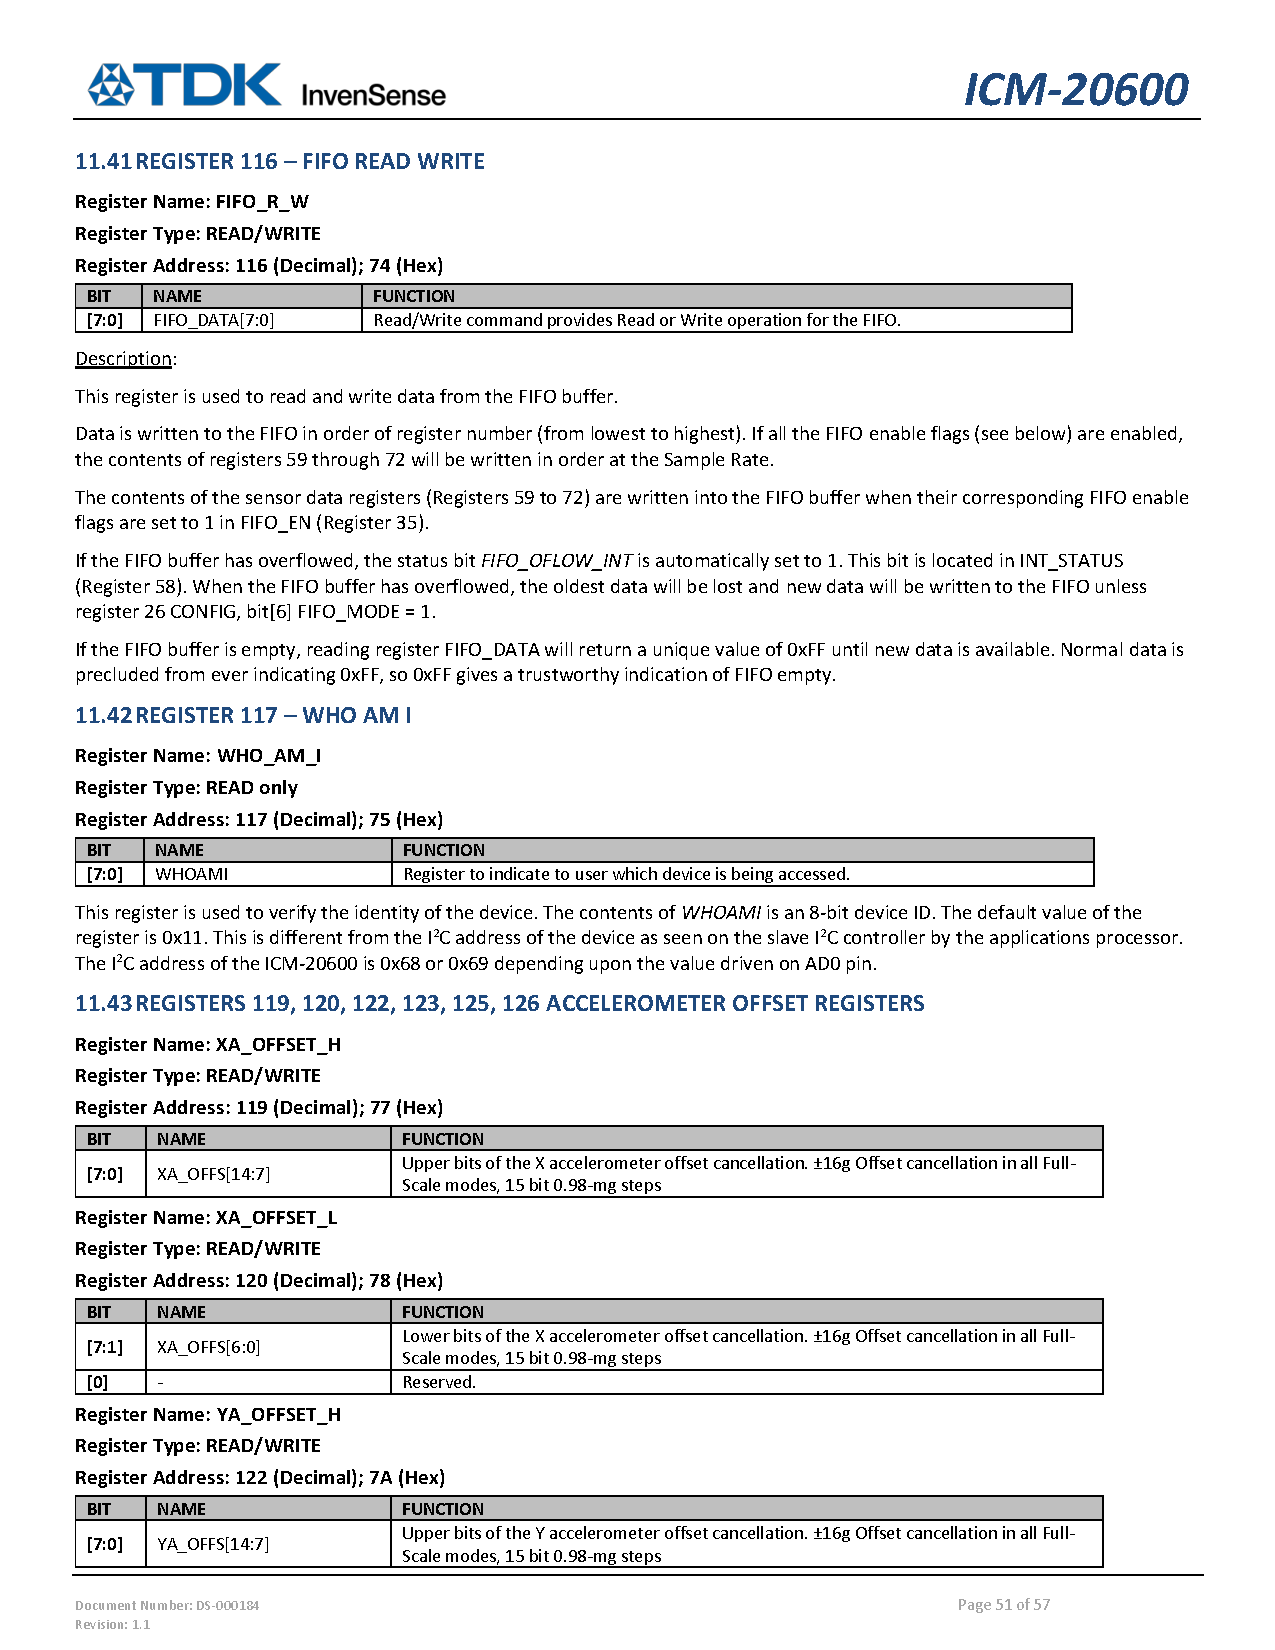
\includegraphics[width=1.1\textwidth]{
		fileForWriting/only two modifiable IIC address}
	\caption[Datasheet of the ICM20600 sensor component.]{Partial datasheet of tthe ICM20600 sensor component~\cite{invensense-icm20600-datasheet}. The No.117 register indicates that for one specific compnent, there are at most two selectable IIC addresses to use.}
	\label{fig:limited-IIC-address}
\end{figure}
%--------End of this FIGURE -----------

\chapter{Codes}

\lstset{language=JavaScript,
	basicstyle=\ttfamily,
	keywordstyle=\color{blue}\ttfamily,
	stringstyle=\color{red}\ttfamily,
	commentstyle=\color{gray}\ttfamily,
	morecomment=[l][\color{magenta}]{\#},
	breaklines=true,
	showstringspaces=false}

\lstset{language=C++}
\lstinputlisting[caption={C\texttt{++} code to init the IIC multiplexer and four sensors.}, label={lst:init-arduino}]{codes/init.cpp}

\lstset{language=C++}
\lstinputlisting[caption={C\texttt{++} code to package the motion data from Arduino into a JSON format.}, label={lst:json-formatter}]{codes/IMU_json.cpp}

\lstset{language=JavaScript,
	basicstyle=\ttfamily,
	keywordstyle=\color{blue}\ttfamily,
	stringstyle=\color{red}\ttfamily,
	commentstyle=\color{gray}\ttfamily,
	morecomment=[l][\color{magenta}]{\#},
	breaklines=true,
	showstringspaces=false}


\lstinputlisting[caption=JavaScript code for flexible-inputting function,label=lst:flexible-input]{codes/flexible-input.js}

\lstinputlisting[caption=JavaScript code for matching and intorpolating data.,label=lst:intorpolation-with-data-matching]{codes/intorpolation-with-data-matching.js}

\lstinputlisting[basicstyle=\footnotesize\ttfamily, breaklines=true, language={}, caption={Log for the Euler angle output in Arduino.},label={lst:time-consuming}]{codes/time-consuming.log}

\lstset{
	basicstyle=\ttfamily,
	keywordstyle=\color{blue}\ttfamily,
	stringstyle=\color{black}\ttfamily,
	commentstyle=\color{gray}\ttfamily,
	morecomment=[l][\color{magenta}]{\#},
	breaklines=true,
	showstringspaces=false}

\lstinputlisting[language=JSON, caption=A text config to generate a model of human lower body.,label={lst:lower-body-config}]{codes/IMU_schedule-lower-body.json}

\lstinputlisting[language=JSON, caption=Another text config to generate a model of full body,label={lst:full-body-config}]{codes/IMU_schedule-full.json}

\end{document}
